% !TEX encoding = UTF-8 Unicode
\documentclass[10pt]{amsart}

%%% MY PACKAGE
\usepackage{mysetup}

\begin{document}
	
	\title{Assignment No. 2: Advanced Methods}
	\author{Studend ID: 10729579}
	\maketitle
	
	\vspace{-0.3cm}
	\setcounter{secnumdepth}{0}
	\section{Introduction}
		\noindent We are supposed to price a bond contract whose terminal condition is given by
%%% TERMINAL CONDITION OF THE BOND PRICE 
\begin{equation}
	V(S,T) = \max \left(F, RS\right).
\end{equation}

Moreover, the issuer of the bond pays out a continuous coupon at the rate of 
\begin{equation}
	K(t) = C \exp{-\alpha t},
\end{equation}
for $\alpha$ and $C$ of his choosing. 

The risk-neutral process followed by underlying stock price is given by
\begin{equation}
	\d S = \kappa \left(\theta(t)  - S\right)\d t + \sigma S^\beta \d W,
\end{equation}
with $\kappa$ being the mean reversion rate, $\beta$ the elasticity of variance in the market, and the function $\theta$ is given by
\begin{equation}
	\theta(t) = (1+\mu)X\exp{\mu t},
\end{equation}
where $X$ and $\mu$ are constant model parameters that can be determined from the market, reflecting the dividend payout of the firm.

The market value $V(S,t)$ of this contract satisfies the following PDE
\begin{equation}\label{general_pde}
	\partial_t V + \frac{1}{2}\sigma^2 S^{2\beta}\partial_{SS}V + \kappa (\theta(t) - S)\partial_SV - rV + C\exp{-\alpha t} = 0,
\end{equation}
where its boundary conditions are given by
\begin{equation}\label{pde_S0}
	\partial_t V + \kappa \theta(t) \partial_S V - rV + C\exp{-\alpha t} = 0, \doublequad \text{ at } S= 0,
\end{equation}
and
\begin{equation}
	V(S,t) = S A(t) + B(t), \doublequad \text{ as } S\to\infty,
\end{equation}
for $A$ and $B$ some functions to be derived.
	
	%& FIRST TASK: EUROPEAN OPTIONS
	\newpage
	\setcounter{secnumdepth}{4}
	\section{European Options}
		\subsection{Derivation of boundary condition for large $S$}
			%& TASK 1: EUROPEAN OPTIONS
\noindent We are told to derive the boundary conditions for (\ref{general_pde}). To do so, we are assuming that 
%%% BOUNDARY CONDITIONS: ASSUMPTION FOR THE SOLUTION OF THE PDE 
	\begin{equation}\label{boundary_condition}
		V(S, t) = S A(t) + B(t) \doublequad \text{ as } S\to \infty,
	\end{equation}
for some functions $A$ and $B$ which solve the approximate problem
%%% THE PDE 
	\begin{equation}\label{pde}
		\partial_t V + \kappa (X - S) \ \partial_S V - rV + C \exp{-\alpha t} = 0
	\end{equation}
obtained after taking $S\to\infty$ in (\ref{general_pde}). We must firstly note~that
	\begin{equation}\label{derivatives}
		\partial_t V (S, t) = S A'(t) + B'(t), \doublequad \text{ and } \doublequad \partial_S V = A(t),
	\end{equation}
to further substitute (\ref{derivatives}) in (\ref{pde}) and get
	\begin{equation}\label{calc1}
		\begin{aligned}
			S A'(t) + B'(t) + \kappa (X - S) A(t) - r \left[ S A(t) + B(t)\right] + C\exp{-\alpha t} = 0.
		\end{aligned}
	\end{equation}

Since the solution is of the form (\ref{boundary_condition}), we may arrange (\ref{calc1}) into something of the same form, that is,
	\begin{equation}\label{calc2}
		\begin{aligned}
			S \left[A'(t) - (\kappa + r) A(t) \right] + \left[ B'(t) + \kappa X A(t) - rB(t) + C\exp{-\alpha t}\right] = 0,
		\end{aligned}
	\end{equation}
which is equivalent to solve
	\begin{equation}
		\begin{cases}
			A'(t) &=  (\kappa + r) A(t) \\
			B'(t) &= rB(t)  - f(t) \\
		\end{cases},
	\end{equation}
where $f(t) = \kappa X A(t) + C\exp{-\alpha t}$.

The first equation gives us that $A(t) = A_T \exp{-(\kappa + r)(T-t)}$, with 
$
A_T \overset{\text{\tiny def}}{=} A(T) \to R,
$ 
as $S\to\infty$. Hence, 
\begin{equation}\label{A}
	A(t) = R\exp{-(\kappa + r)(T-t)}
\end{equation} 

On the other hand, second equation gives us that $B$ is of the form $B(t) = C(t) \exp{-r (T-t)}$, $C(T) = B(T)$, where $C(t)$ is to be derived. Differentiating $B(t)$ and rearranging terms we get
%%% ODE FOR THE "CONSTANT" MULTIPLYING B
	\begin{equation}\label{C_ode}
		C'(t) = - \exp{r(T-t)}f(t), 
	\end{equation}
with $  B_T \overset{\text{\tiny def}}{=} B(T) $, which is zero for large $S$, i.e.,
	\begin{equation}\label{C_ode_sol}
		 C(t) 	= B_T + \int_t^T \exp{r(T-s)}f(s)\d s,
	\end{equation}
which implies that (see Appendix \ref{app_ODE_C})
	\begin{equation}
		C(t) = B_T + {X R}  \left[1 -  \exp{-\kappa(T-t)}\right]- \frac{C}{r+\alpha}\exp{rT}\left[\exp{-(r+\alpha)T}-\exp{-(r+\alpha)t}\right]
	\end{equation}

Therefore, for $S$ sufficiently large we obtain (see Appendix \ref{app_ODE_C}),
	%%% B(t) 
	\begin{equation}\label{B}
			B(t)  = {2X R}\exp{-\left(r+\frac{\kappa}{2}\right)(T-t)}\sinh\left(\frac{\kappa}{2}[T-t]\right)- \frac{C}{r+\alpha}\exp{rt}\left[\exp{-(r+\alpha)T}-\exp{-(r+\alpha)t}\right]
	\end{equation}

Finally,
	%%% VALUE FUNCTION WHEN S TENDS TO INFINITY
	\begin{equation}\label{boundary_formula}
		V(S,t) = SR  \ \exp{-\kappa_r(T-t)} +  {2X R}\exp{-\frac{1}{2}\left(r-\kappa_r\right)(T-t)}\sinh \frac{\kappa}{2}(T-t)- \frac{C}{\alpha_r}\exp{rt}\left[\exp{-\alpha_r T}-\exp{-\alpha_r t}\right],
	\end{equation}
	where $\kappa_r \defi \kappa + r$, and $\alpha_r \defi  \alpha + r.$

		\subsection{Crank Nicolson Scheme}
			As we are told to do, we have used the Crank-Nicolson scheme to calculate the value of the option.

To do so, we have calculated an analytic solution for $V$ both when $S=0$ and $S$ becomes large, in order to set the boundary conditions up, i.e., $a[0], b[0], c[0], d[0]$ and $a[\texttt{m\_J}], b[\texttt{m\_J}], c[\texttt{m\_J}], d[\texttt{m\_J}]$, with \texttt{m\_J} being the member variable of the class \texttt{CCrackNicolson} which can be found in the files \texttt{CCrackNicolson.cpp} and \texttt{CCrackNicolson.h}, and which gives us the distance between the stock prices of the grid, i.e.,  $\texttt{m_dS} = \texttt{m_Smax} / \texttt{m_J}$ . The derivation of $V(S=0, t)$ using the method of characteristics for first-order partial differential equations can be found in the Appendix \ref{app_bound_V_S0}:
\begin{equation}\label{V_S0}
	V(S=0,t) =  F \exp{-r(T-t)} + \frac{C}{r+\alpha} \exp{-\alpha T}\left( \exp{\alpha (T-t)} -\exp{-r(T-t)} \right).
\end{equation}

On the other hand, the derivation of the coefficients can be found in the Appendix \ref{app_coeff_CrankNic}, and are given by 
\begin{equation}
	\begin{aligned}
		a(j) &= -\frac{1}{4}\sigma^2j^{2\beta}(\Delta S)^{2(\beta -1) }+ \frac{\kappa}{4}\left[\frac{\theta(\Delta t)}{\Delta S} - j\right] \\
		b(j) &= \frac{1}{\Delta t} + \frac{r}{2} + \frac{1}{2}\sigma^2 j^{2\beta}(\Delta S)^{2(\beta -1) }\\
		c(j) &=  -\frac{1}{4}\sigma^2j^{2\beta}(\Delta S)^{2(\beta -1) } - \frac{\kappa}{4}\left[\frac{\theta(\Delta t)}{\Delta S} - j\right]\\
		d(i,j)&=\left(\frac{1}{4}\sigma^2 j^{2\beta}(\Delta S)^{2(\beta -1) } - \frac{\kappa}{4}\left[\frac{\theta(\Delta t)}{\Delta S} - j\right]\right)V_{i+1,j-1}\\
		&+ \left(\frac{1}{\Delta t } - \frac{1}{2}\sigma^2 j^{2\beta}(\Delta S)^{2(\beta -1) }  - \frac{r}{2}\right)V_{i+1,j}\\
		&+ \left(\frac{1}{4}\sigma^2 j^{2\beta}(\Delta S)^{2(\beta -1) }+ \frac{\kappa}{4}\left[\frac{\theta(\Delta t)}{\Delta S} - j\right]\right)V_{i+1,j+1} + C \exp{-\alpha \Delta t}.
	\end{aligned}
\end{equation}
for all $0< j < \texttt{m_J}$.

For $j=0$ and $j = \texttt{m_J}$ we set $a[0] = c[0] = a[\texttt{m\_J}] = c[\texttt{m\_J}] =  0$ and $b[0] = b[\texttt{m\_J}] = 1$ because we have an analytic solution for both cases. More precisely, in the $i$th step, $\texttt{d[0]} = \texttt{V_S0}[(i + 0.5) * \texttt{m_dt}]$, where $\texttt{m_dt} = \texttt{m_T} / \texttt{m_I}$, with $m_T$ the time to maturity (in our case is $T=3$) and $\texttt{m_I}$ is the number of time steps we want in our grid. The function $\texttt{V_S0}$ can be found in the class $\texttt{CConvertibleBonds}$ within the files \texttt{Convertiblebonds.cpp} and \texttt{ConvertibleBonds.h}.

Analogously, in the $i$th step, $d[\texttt{m_J}] = \texttt{V_Smax}(\texttt{m_Smax, (i + 0.5) * \texttt{m_dt}})$, where he function $\texttt{V_Smax}$ can be found in the class $\texttt{CConvertibleBonds}$ within the same two files.

In other words, for all $i$,
\begin{equation}
	\begin{aligned}
		d(i,0) &= F \exp{-r(T-(i + 0.5) \Delta t)} + \frac{C}{r+\alpha} \exp{-\alpha T}\left( \exp{\alpha (T-(i + 0.5) \Delta t)} -\exp{-r(T-(i + 0.5) \Delta t)} \right),\\
		d(i,J) &= Smax \ A((i + 0.5) \Delta t) + B((i + 0.5) \Delta t),
	\end{aligned}
\end{equation}
where $A$ and $B$ are the functions given in (\ref{A}) and (\ref{B}).



		\subsection{Value of the option at $t=0$ as a function of $S$.}
			In this task we are aim to find the value of the option, $V(S,t)$ as a function of the underlying asset price $S$ at $t=0$, i.e., $V(S,t=0)$. In order to so, we are given two pairs of specific values of $\beta$ and $\sigma$. 
\begin{enumerate}[wide, labelindent=1cm]
	\item $\beta=1$ and $\sigma = 0.381$, and all other parameters as standard.
	\item $\beta=0 0.808$ and $\sigma=0.66$, and all other parameters as standard.
\end{enumerate}
\vspace{-0.3cm}
\begin{figure}[htbp]
	\centering
	\captionsetup{width=.5\linewidth}
	\begin{subfigure}[b]{0.49\textwidth}
		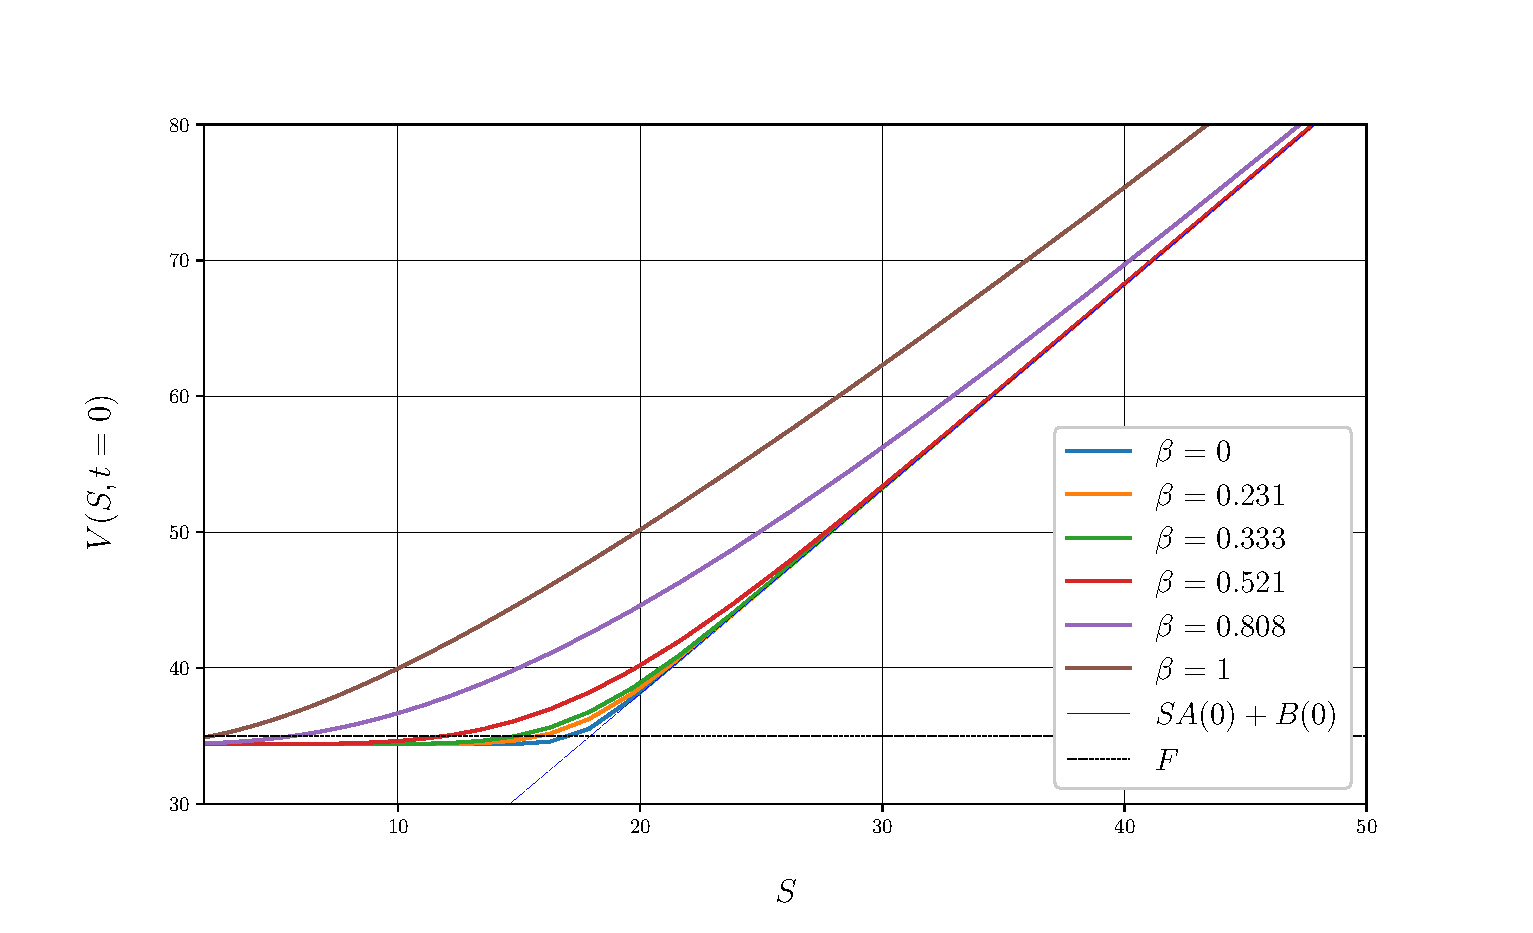
\includegraphics[width=\textwidth]{img/Q1/ComparisonDifferentBetas_sigma06600.eps}
		\captionsetup{width=.8\linewidth}
		\caption{Value of the option for different $\beta$ as $S$ becomes larger with $\sigma = 0.381$.}
		\label{changingBeta}
	\end{subfigure}
	\begin{subfigure}[b]{0.49\textwidth}
		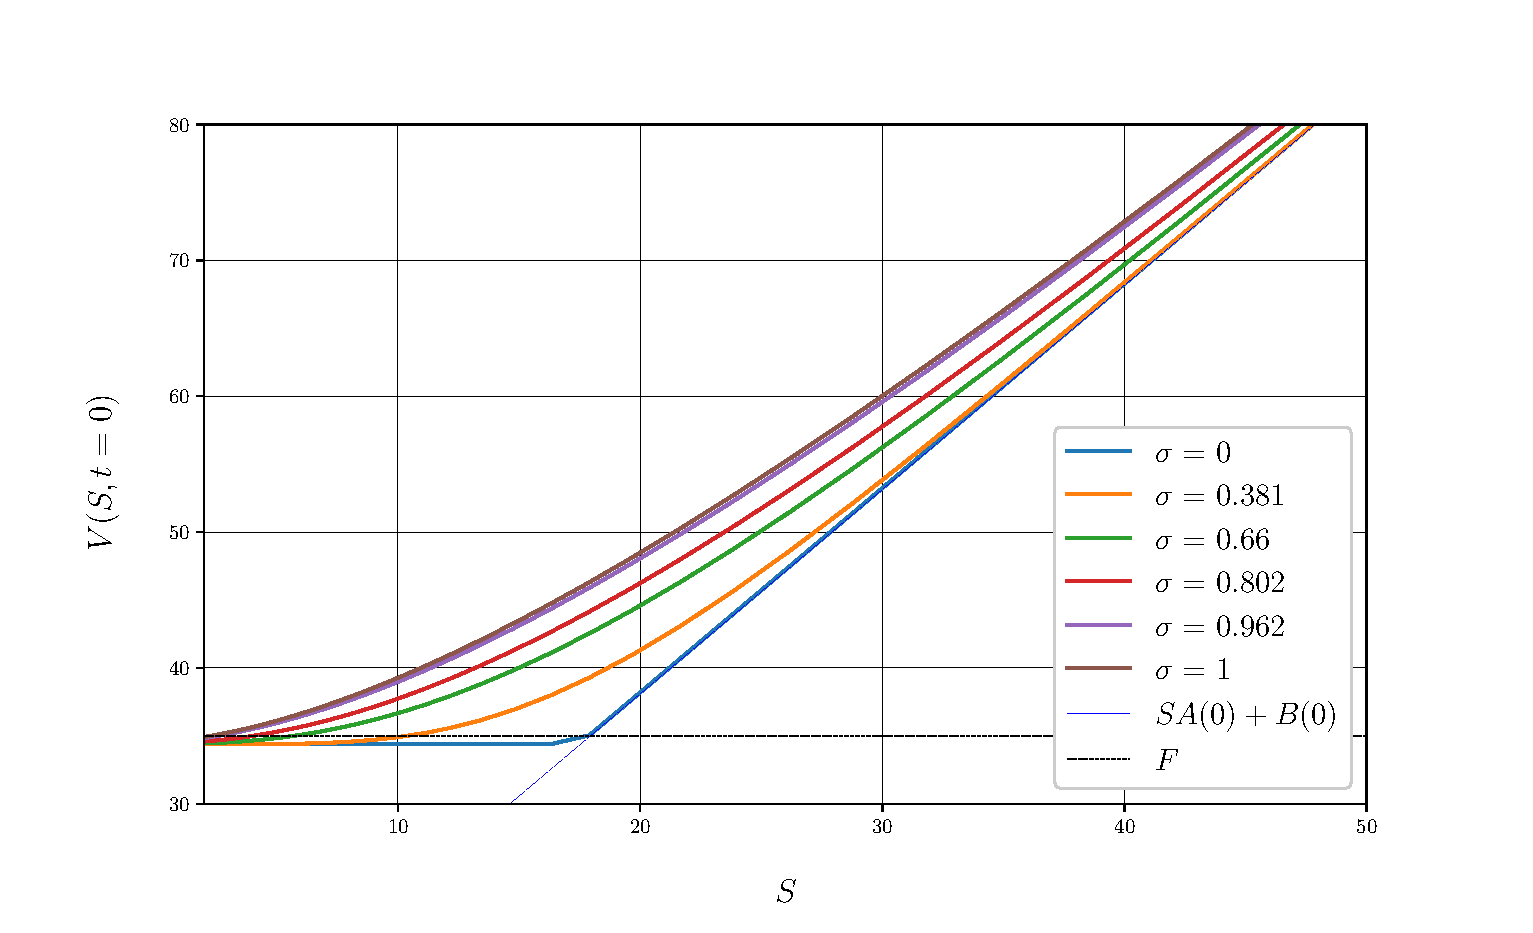
\includegraphics[width=\textwidth]{img/Q1/ComparisonDifferentSigmas_beta0808.eps}
		\captionsetup{width=.8\linewidth}
		\caption{Value of the option for different $\sigma$ as $S$ becomes larger with $\beta=0.808$.}
		\label{changingSigma}
	\end{subfigure}
	\caption{Value of the option as $S$ becomes larger for different parameters.}
	\label{S_larger}
\end{figure}
\vspace{-0.3cm}
The idea is to see what happens when $\beta$ and $\sigma$ are changed, so firstly let's plot some graphs with a few values of $\beta$ and $\sigma$. We have chosen six values for both parameters from $0$ to $1$ (including them). In Figure \ref{changingBeta}, $\sigma$ is fixed, whilst $\beta$ is fixed in Figure \ref{changingSigma}. But firslty we are trying to understand theoretically what's going on. On the one hand, both $\beta$  and $\sigma$ contribute to the term 
\begin{equation}
	\frac{1}{2}\sigma^2S^{2\beta}\partial_S^2 V.
\end{equation}

Moreover, note from (\ref{general_pde}) that
\begin{equation}
	V = \frac{1}{r}\left(\partial_t V + \frac{1}{2}\sigma^2 S^{2\beta}\partial_{SS} V + \kappa\left(\theta(t) - S\right)\partial_S + Ce^{-\alpha t}\right);
\end{equation}
which means that, when all of the parameters are the same but not $\beta$ and $\sigma$, then we can understand $V(S,t)$ as
\begin{equation}\label{useful}
	V = \frac{1}{2r}\sigma^2 S^{2\beta}\partial_{SS} V + \text{other}.
\end{equation}

On the other hand, we know that when $S$ becomes larger, $V(S,t)$ tends to $S A(t) + B(t)$, so the contribution of $\beta$ and $\sigma$ is significant when $S$ is somehow small. Moreover, it is obvious from (\ref{useful}) that $V$ becomes smaller as $\sigma$ and $\beta$ becomes smaller. Particularly, when $\beta \to 0$, then
\begin{equation}
	V \to  \frac{1}{2r}\sigma^2\partial_{SS} V + \text{other};
\end{equation}
and, when $\sigma\to 0$, 
\begin{equation}
	V \to  \text{other},
\end{equation}
and the contribution of the second derivative with respect of $S$ is null, i.e., it's (locally) linear on $S$ (tending to $F$ for small $S$). This is coherent with Figure \ref{S_larger}, in which we can see how the value of the option flattens before the cross of $F$ and $S A(0) + B(0)$, i.e., when
\begin{equation}
	S^* = \frac{F-B(0)}{A(0)} = 17.94670.
\end{equation} 

This means that when $S < S^*$, then $V(S,0) \to F$ as $\sigma, \beta\to0$. Intuitively speaking, $\sigma$ is the volatility of the process, so the larger the sigma, the larger the random fluctuation from the Brownian Motion. In some sense, it increases the randomness of the stock price. On the other hand, $\beta$ can be understood as the elasticity of the stock price, meaning that $\sigma S^\beta$ is the instantaneous volatility of the stock price, i.e., 
\begin{equation}
	\frac{\partial_S \left(\sigma S^\beta\right)}{\sigma S^{\beta}/S} =\frac{\sigma \beta S^{\beta-1}}{\sigma S^{\beta-1}} = \beta,
\end{equation}
which means that it is the percentange of change in instantaneous volatility as $S$ changes. If $\beta < 1$, the volatility increases as the stock price decreases, and viceversa, but not monotonically: since $\sigma S^{\beta}$ is a concave function on $S$, then de increasing is faster for smaller $S$.

\begin{figure}[htbp]
	\centering
	\captionsetup{width=.5\linewidth}
	\begin{subfigure}[b]{0.49\textwidth}
		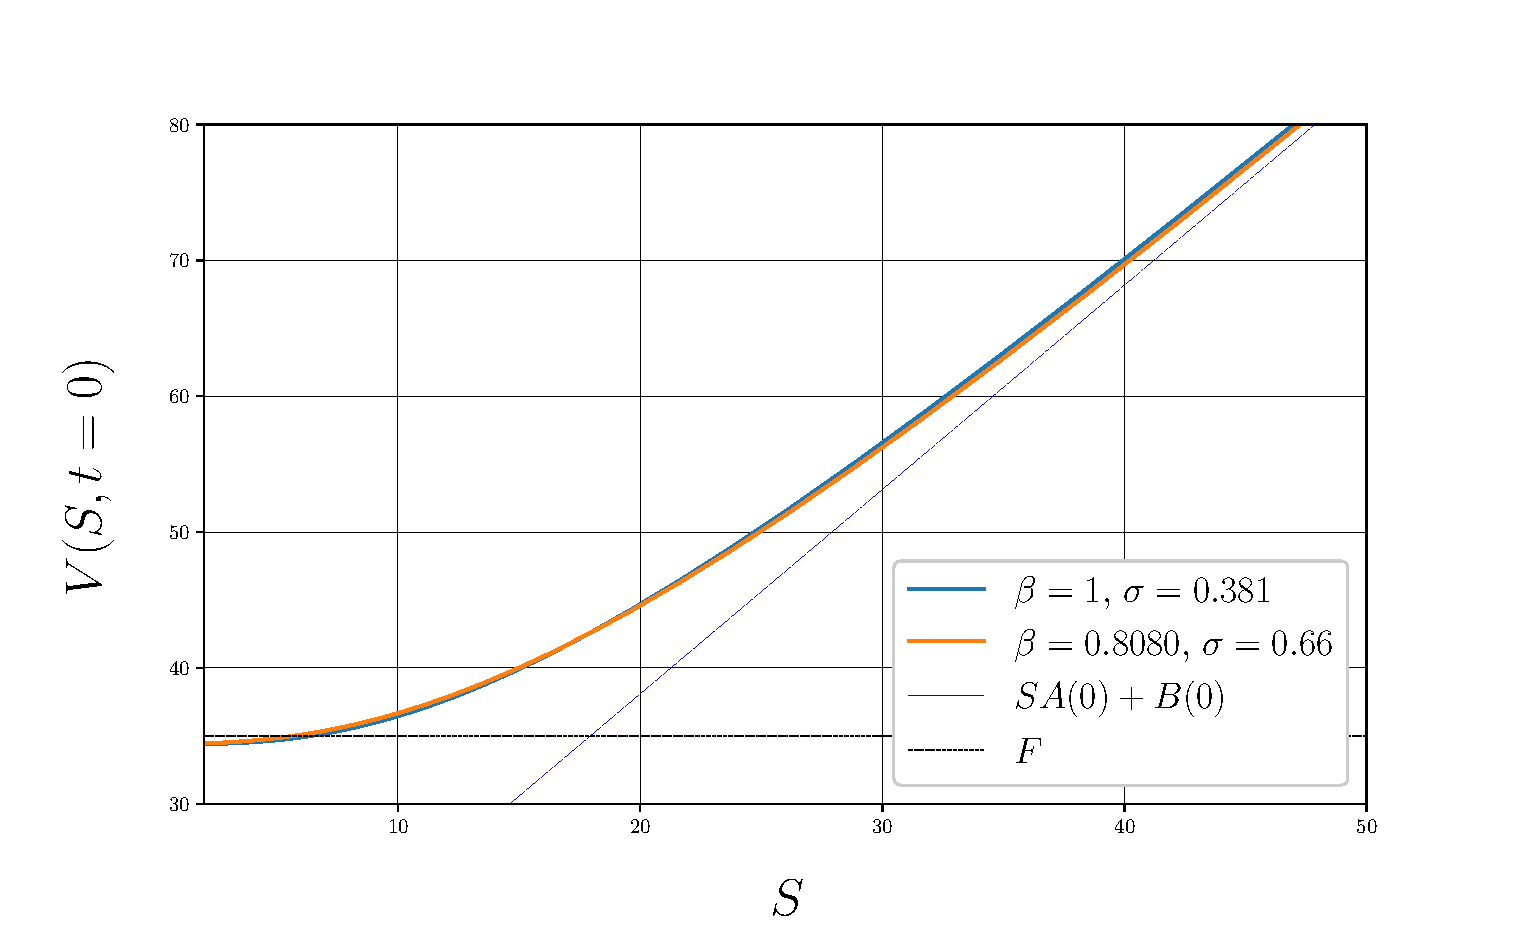
\includegraphics[width=\textwidth]{img/Q1/ComparisonGivenBetaAndSigma.eps}
		\captionsetup{width=.8\linewidth}
		\caption{Value of the option for different $\beta$ as $S$ becomes larger with $\sigma = 0.381$.}
		\label{withoutZoom}
	\end{subfigure}
	\begin{subfigure}[b]{0.49\textwidth}
		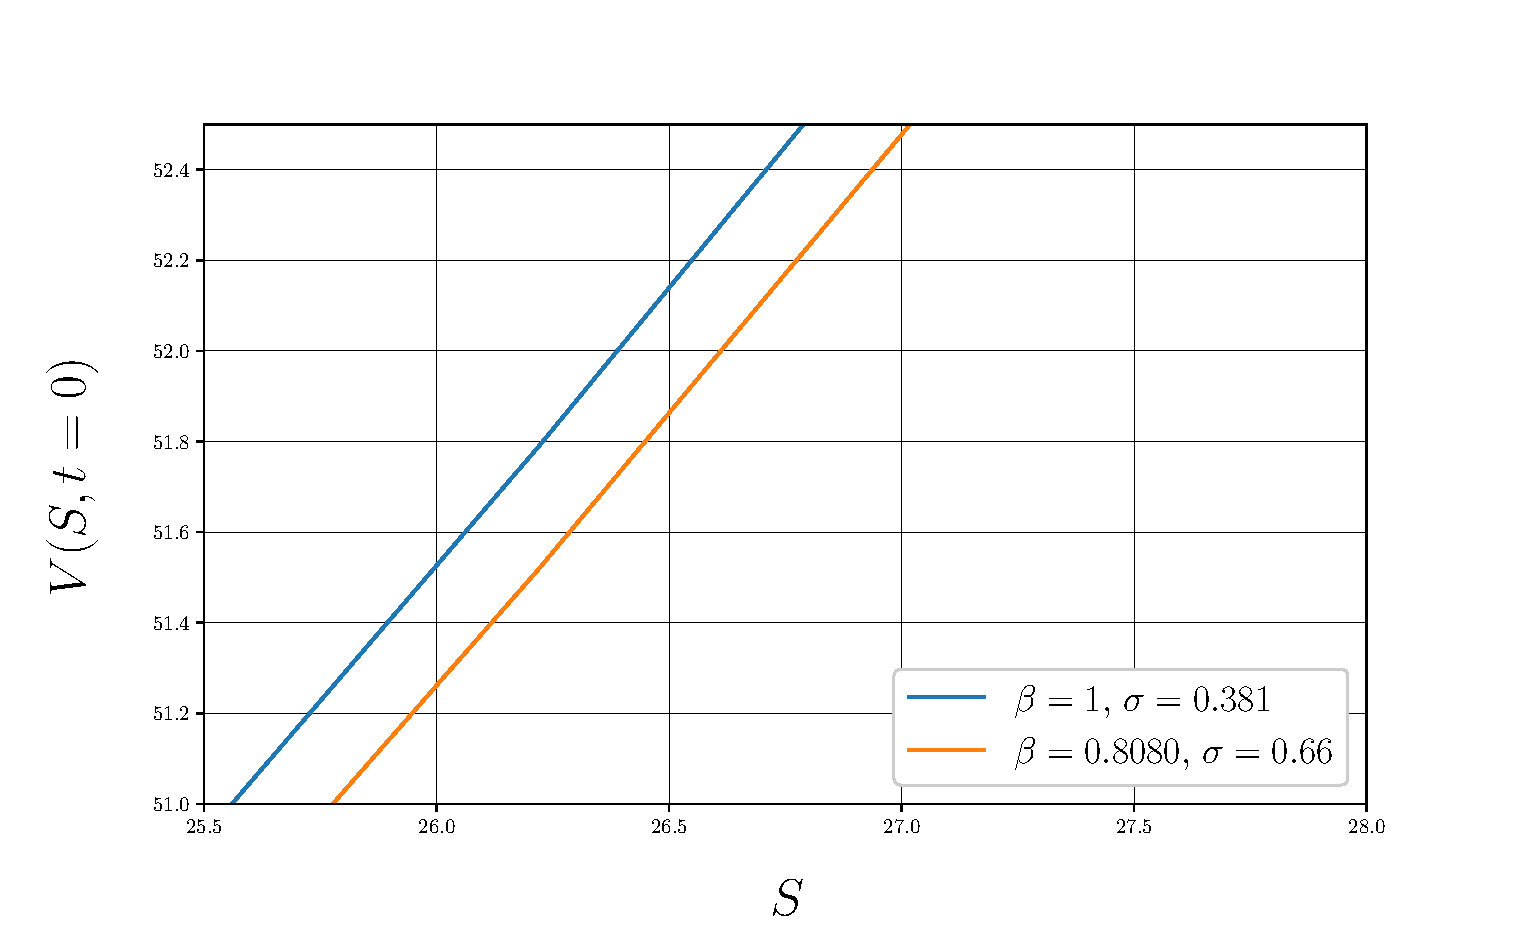
\includegraphics[width=\textwidth]{img/Q1/ComparisonGivenBetaAndSigmaZoom.eps}
		\captionsetup{width=.8\linewidth}
		\caption{Value of the option for different $\sigma$ as $S$ becomes larger with $\beta=0.808$.}
		\label{withZoom}
	\end{subfigure}
	\caption{Value of the option as $S$ becomes larger for different values of parameters $\beta$ and $\sigma$.}
	\label{StudyingBetaSigma}
\end{figure}

In particular, we are told to study the option option value when $\beta=1$ and $\sigma = 0.381$ and $\beta=0.808$ and $\sigma=0.66$. As we can see in Figure \ref{withoutZoom}, the results are nearly the same, just separated by a difference of $0.2$ (see the Figure \ref{withZoom}). This means that a relatively low $\sigma$ is compensated with a relatively big $\beta$ and viceversa. Moreover, all the solutions will converge to the same line, because  (\ref{boundary_formula}) does not depend on $\beta$ and $\sigma$. Hence, the role of $\beta$ and $\sigma$ is just to determine how fast the solution converges to $SA(0) + B(0)$ for $S>S^*$ and how plattened it is when $S<S^*$.



		\subsection{Value of the option when $S_0=17.38$.}
			In this task we have to find the value of the option when $S_0 = 17.38$, and $\beta = 0.808$ and $\sigma  = 0.66$. To do so, we set a squared-grid, i.e., $\texttt{m_J} = \texttt{m_I} = N$ and obtain different values (first column of the next tables). From a first sight, we can roughly see that the value of the option when $S_0 = 17,38$ is around $42.05\pm10^{-2}$. However we would like to see how much we could improve our result to get more digits of precision. This can be done by increasing $S_{max}$. The idea is to have $S_0$ within the points of the grid, although we can make use of Lagrange Interpolation (of different degrees) to make sure we have a correct result. However, this would add some errors, and it is desiderable to avoid them. The idea is therefore to make sure that there exists a $j^*$ such that $S_0 = j^* \Delta S$, where $\Delta S = S_{max} / J$. Therefore, $j^* = \frac{S_0 J}{S_{max}}$ but, in our case, we have that $X = S_0$, so an easy way to make $J$ an integer is to take $S_{max} = k X$. This would imply that $J =  k j^*$ for some integer $k$. On the other hand, in order to study the convergence, we must iterate the method with different $J$. To do so, we have done a loop ``\texttt{for (int n=nMin; n<=nMax; n*=incr)}'' with $\texttt{nMin=3, nMax=50000, incr=2}$ (they could have been different) and with $\texttt{I=J=n*ceil(Smax/S0)=n*k}$. We can see an example in Table \ref{table1}.

\begin{table}[h!]\scriptsize
	\setlength{\tabcolsep}{5pt}
	\renewcommand{\arraystretch}{1.3}
	\begin{tabular}{c|ccccccccc}
		\hline\addlinespace[0.1cm]
		I=J			& 48	& 96 & 192 & 384 & 768 & 768 & 1546 & 2072 & 6144 \\
		$V(S_0,0)$ & 41.8408512 & 42.004891854 & 42.04124385 & 42.04867403 & 42.04973806 & 42.049609 & 42.04957 & 42.0495647 & 42.049562 
       \\\addlinespace[0.1cm]
		\hline
	\end{tabular}
	\vspace{0.3cm}
	\captionsetup{width=.55\linewidth}
	\caption{Values when increasing $\texttt{m_I}$ and $\texttt{m_J}$, Lagrange Interpolation of degree $16$ and $S_{max} = 8X$.}\label{table1}
\end{table}
\vspace{-0.6cm}
In order to improve our results and get more efficiency using a lower $J$, we can study the convergence of our values to further use Richardson Extrapolation (maybe more than one time). The ratios of the difference between results\footnote{Given three values $v_1$, $v_2$, $v_3$, we define the ratio between their differences as $\frac{v_2-v_1}{v_3-v_2}$. Since the convergence of Crank Nicolson method is $\mathcal{O}((\Delta S)^2, (\Delta t)^2)$, then we expect this ratio to be $4$, because the increments are produced by doubling $J$.} can be found in Table \ref{table2}.

\begin{table}[h]\scriptsize
	\setlength{\tabcolsep}{8pt}
	\renewcommand{\arraystretch}{1.3}
	\begin{tabular}{r|rrrrrrrrrr}
		\hline\addlinespace[0.1cm]
		$V(S_0,0)$ & 4.51256 & 4.89249 & 6.98301 &  8.26535 & 3.47294 & 4.95559 & 2.69404 & 9.72845 & 0.97506 & \\
		I Extrap & 2.80979 & 2.08924 & 2.01019 & 80.82043 & 2.73326 & 1.97126 & 2.21787 & 1.84651 & 2.29676 &          \\\addlinespace[0.1cm]
		\hline
	\end{tabular}
	\vspace{0.2cm}
	\captionsetup{width=.55\linewidth}
	\caption{Ratios from Table \ref{table1} and after doing one extrapolation with $p=2$.}\label{table2}
\end{table}
\vspace{-1cm}
As we can see, the ratios are not stricly monotonic, but the majority of them are near $4\pm1$, so we can try to do Richardson Extrapolation in order to try to get a more accurate result in less time. Richardson extrapolation provides, from a method of order $p$, an extrapolated result $v_{extrap}$ which can be found in the second row of Table~\ref{table2} and which is given by
\begin{equation}
	v_{extrap} = \frac{2^p v_{new} - v_{old} }{2^p - 1}.
\end{equation}

This can be repeated a second time in order to get a new extrapolated value\footnote{We have not obtained a better approximation but the confirmation of at lteast $4$ digits (42.0495) when $I=J=1536$ and of six digits (42.049561) when $I=J=24576$.}, but this time with $p=1$, because the order is $1$ after one extrapolation, as we can see in Table \ref{table2}. Finally, we have kept the values of the contract as $I, J$ increase and after two extrapolations (with $p=1$) in Table \ref{table3}, with $S_{max} = 8X$\footnote{Other values of $S_{max}$, like $4X$, $16X$ and $32X$, have been tried, but none of them has provided a better convergence ratio than $8X$, so we have decided to include only a table for $S_{max}=8X$ in order to not being repetitive.}.

\begin{table}[h!]\scriptsize
	\setlength{\tabcolsep}{15pt}
	\renewcommand{\arraystretch}{1.2}
	\begin{tabular}{rrrrl}
	I& J&   $V(S_0,0)$		& 1st Extrapolation & 2nd Extrapolation\\\hline
	   48 &    48 & 42.0048918538 & 42.0595720633 & -                                     \\
	96 &    96 & 42.0412438594 & 42.0533611946 & 42.047150325933316 \\
	192 &   192 & 42.0486740302 & 42.0511507538 & 42.048940312999996  \\
	384 &   384 & 42.0497380652 & 42.0500927435 & 42.04903473326667  \\
	768 &   768 & 42.0496093308 & 42.0495664193 & 42.04904009513334   \\
	1536 &  1536 & 42.0495722630 & 42.0495599071 & 42.04955339480001    \\
	3072 &  3072 & 42.0495647830 & 42.0495622897 & 42.04956467226666   \\
	6144 &  6144 & 42.0495620065 & 42.0495610810 & 42.04955987233335    \\
	12288 & 12288 & 42.0495617211 & 42.0495616260 & 42.04956217093333  \\
	24576 & 24576 & 42.0495614284 & 42.0495613308 & 42.049561035700016   \\
	49152 & 49152 & 42.0495614516 & 42.0495614593 & 42.04956158783331  \\
	\end{tabular}
	\vspace{0.2cm}
	\captionsetup{width=.55\linewidth}
	\caption{Values when increasing $\texttt{m_I}$ and $\texttt{m_J}$, Lagrange Interpolation of degree $16$ and $S_{max} = 8X$.}\label{table3}
\end{table}
\vspace{-0.5cm}
From this table we can conclude that the $V(S_0,0)$ converges to $42.049561$ as $I$ and $J$ increases. However, when $I = J \geq 16384$, the time consumption is too high. To reduce it, we just can get three values using $I= J \in \{3072,6144\}$ and do the extrapolation of order $2$. Since $3072+6144 = 9216 < 12288$, we can obtained six digits of precision with 3072 iterations less and in $8.979847 + 36.19612 = 45.175967$s, $126.9858$s less than when using $I = J = 12288$, whose result is obtained in $172.1617889$s (extrapolation time is near 0).

If we would want to have just five digits of precision, we could either use $I=J= 3072$ with no extrapolation (8.979847s) or $I=J=384$ (0.1666s) and $I=J=568$ (0.6226s), i.e. 952 iterations (2120 less iterations)  and 0.7892s (less than 1s).

To sum up, we can see in Table \ref{table4} the best results we've got when using $S_{max}\in\{8X,12X\}$. We can definitely say that $V(S,t=0) \approx 42.095$, and that $V(S,t=0) \approx 42.0956\pm 10^{-5}$. To obtain this result, the fastest way is to use $N=1280$, $S_{max} = 12X$ and two extrapolations.
\begin{table}[h!]
	\setlength{\tabcolsep}{12pt}
	\renewcommand{\arraystretch}{1.25}
	\begin{tabular}{c||cc||cc}
		 I, J		&  	Value & Time (s)& Extrapolated Value& Time (s)\\\hline\addlinespace[0.05cm]
		952 	& 	42.04953 & 1.3855&42.04956 	& 0.7892 \\
		9216 	&	42.049560& 106.5886&42.049561 	& 126.9858 \\
	\end{tabular}
\vspace{0.25cm}
	\captionsetup{width=.639\linewidth}
	\caption{Values of the contract when using directly Crank Nicolson and using two different values to obtain the extrapolated value with $p=2$.}\label{table4}
\end{table}
\vspace{-0.5cm}
Finally, just mentioned that ratios of the differences between values may give us the convergence rate, which is theoretically $O((\Delta t)^2, (\Delta S)^2)$. Since they are the same and we have increases of $2n$, we expect to have ratios around $4$. For example, for $S_{max}$, the ratios we've obtained are given in Table \ref{table2}. As we can see, the ratios are not always $4$, so we may not expect the extrapolatino to be perfect. However, as we have mentioned before, many ratios are near to $4$, and indeed the extrapolation has provide us with good result, as we can see in Table \ref{table4}

	\vspace{1cm}
	%& SECOND TASK: AMERICAN OPTIONS - EMBEDDED OPTIONS
	\newpage
	\section{American Options - embedded put option}
			In order to find the value of the contract with an embedded put option, we have decided to use the Penalty Method. This method consists in adding a ``pushing'' term in the PDE (\ref{general_pde}), which in our case depends on two conditions that must be satisfied due to the proper definition of our contract. Briefly speaking, this term pushes back toward the exercise value when it's crossed. Moreover, since in our case $b_j > 0$ by definition, then this term must be positive. The code consists in creating new vectors $\texttt{aHat(a)}$, $\texttt{bHat(b)}$, $\texttt{cHat(c)}$, $\texttt{dHat(d)}$, update them with the code given in Figure \ref{codePenalty}, and find $\texttt{y = thomasSolve(aHat,bHat,cHat,dHat)}$ in order to get the new $\texttt{vNew}$ (more details can be found in the Appendix \ref{app_code}).
\vspace{-0.5cm}
\begin{figure}[h!]
\begin{lstlisting}
	if(vNew[j] < m_R*S[j])
	{
		bHat[j] = b[j] + m_rho;
		dHat[j] = d[j] + m_rho*(m_R*S[j]);
	}
	if( approx_t < m_t0 && vNew[j] < m_P)
	{
		bHat[j] = bHat[j] + m_rho;
		dHat[j] = dHat[j] + m_rho*m_P;
	}
\end{lstlisting}
\captionsetup{width=.6\linewidth}
\caption{Code lines for the ppenalty method conditions which update the \texttt{a}, \texttt{b}, \texttt{c}, \texttt{d} coefficients of Crank Nicolson scheme.}\label{codePenalty}
\end{figure}
		\subsection{First analysis of the value of the contract: finding the optimal decision points.}
			In this section we just provide a graph in which we can see the evolution of the value of the contract as $S$ increases (Figure \ref{optimalPoints}). Moreover, we mark on this graph the two optimal decision points: $S_1 = 5.85$ and $S_2 = 35.58$. These two points define three regions where we would take different decisions. 

The first region is defined by $S<S_1$. Here we would sell the bond back to the issuer at $P_p=38$. In the second region, $(S_1,S_2)$, we would hold the contract. Finally, in the third region, $S_2 <\infty$, we would exercise the option and convert the bond in stock.
\vspace{-0.4cm}
\begin{figure}[h!]
	\centering
	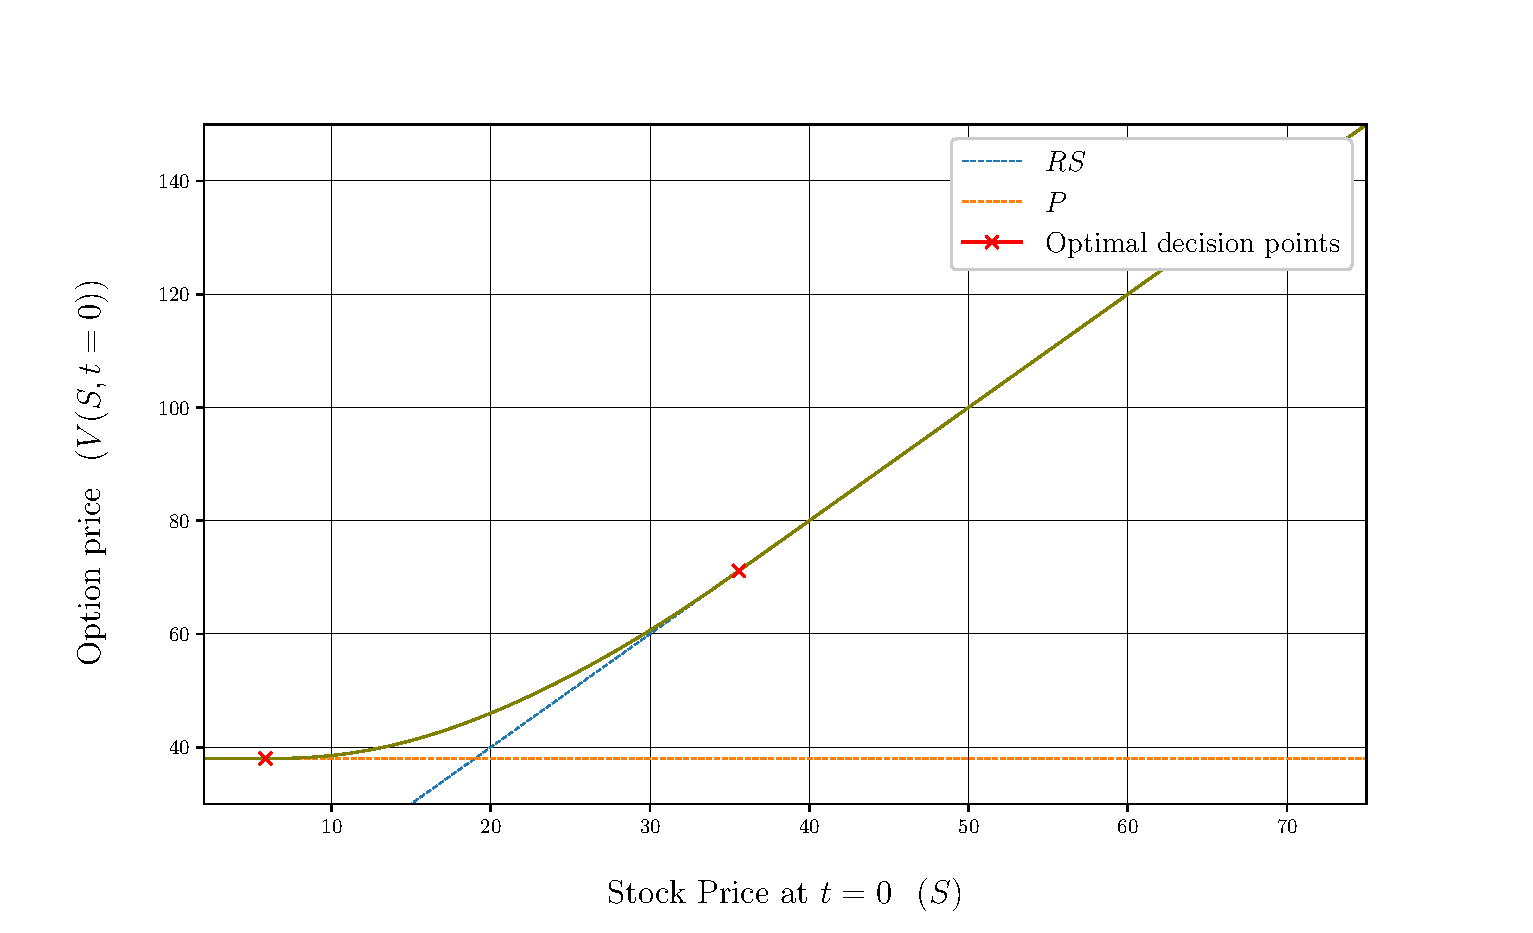
\includegraphics[scale=0.43]{img/Q2/amConvBondValues_incrS_OptimalDecisionPoints}
	\caption{Value of the contract with $r\in\{0.0058,0.0117,0.0175\}$ as $S$ increases.}\label{optimalPoints}
\end{figure}
\vspace{-0.4cm}
		\subsection{Value of the contract with an embedded put option with $r\in\{0.00585, 0.0117, 0.01755\}$ as $S$ increases.}
			In this section we are supposed to explain the behaviour of the value of the contract with for three different values of $r$. Firstly, let's plot out a graph in which we can see the behaviour of the value of the option as $S$ increases, as we are told to do. This can be found in Figure \ref{analysisDifferent_r_withoutZoom}. However, we do not see a great different between the three lines: only in $S\in[10,30]$ seems to be a different behaviour, exactly within the region where the contract is held. Hence, in order to provide a better analysis about the behaviour of this contract with the different $r\in\{0.0058,0.0117,0.0175\}$, we have plotted the value of the contract when $S\in[18,24]$. We can see that the value increases as $r$ decreases. This can be explained by looking at (\ref{useful}): the three values of the contract are given by a fraction in which the numerator is common among all of them and the denominator consists of a product of $r$ with a constant. Hence, it's obvious that as $r$ decreases, then the value of the contract increases.

On the other hand, the $r$ only appears one time in all the formul\ae \ (where we have described). Therefore, the contribution of a slight change in $r$ will provide also a slight change in $V$.
\begin{figure}[h]
	\centering
	\begin{subfigure}[t]{0.5\textwidth}
		\centering
		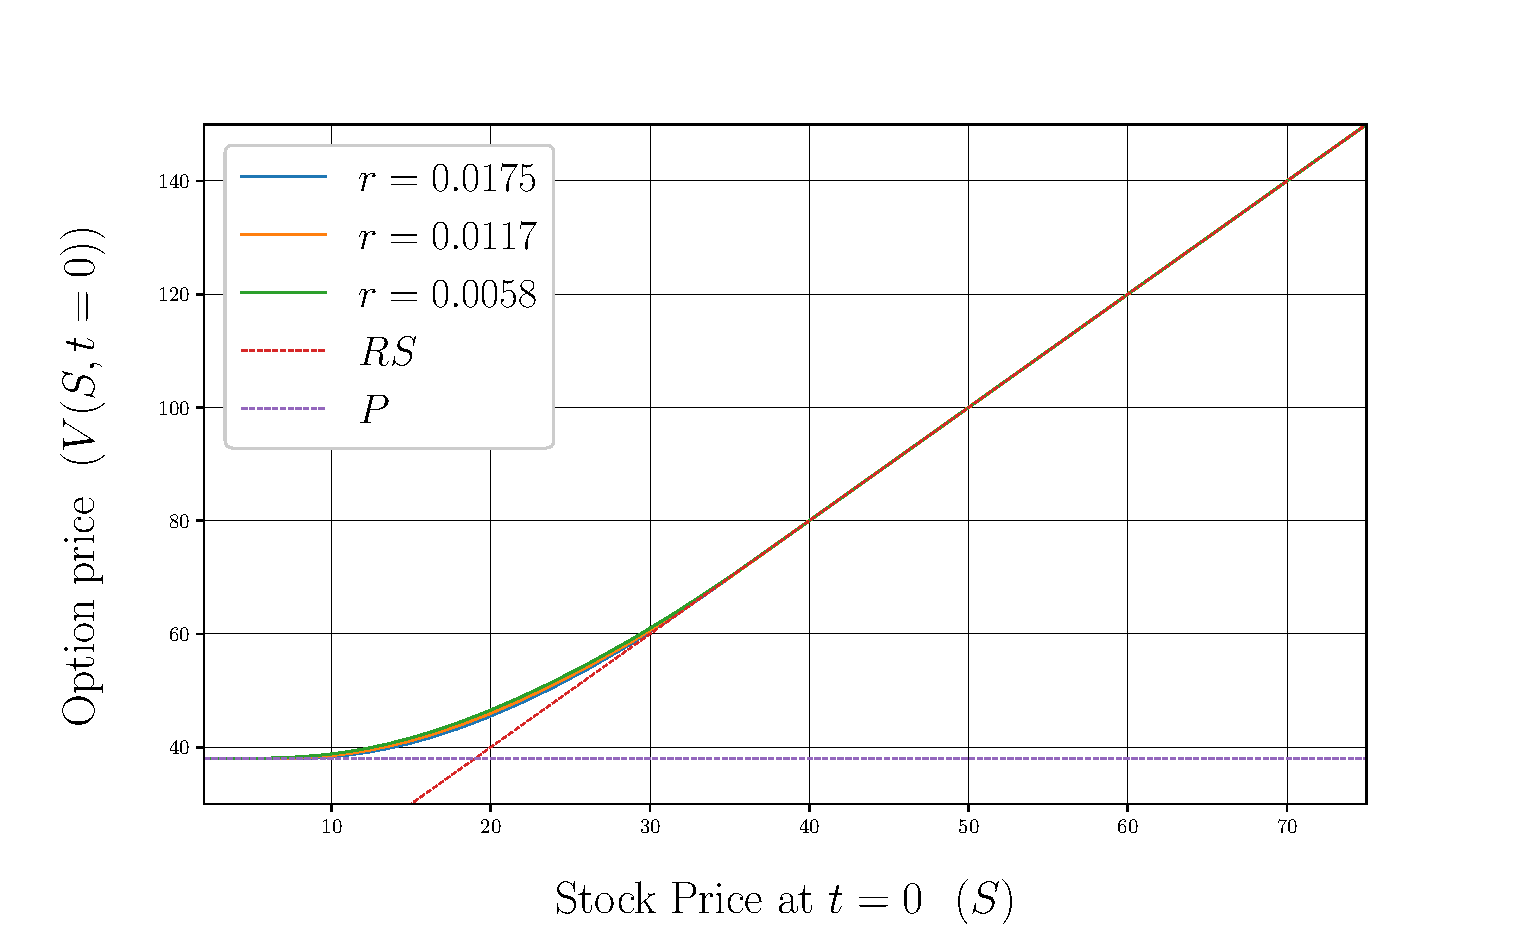
\includegraphics[scale=0.36]{img/Q2/amConvBondValues_incrS_DifferentInterestRates}
		\captionsetup{width=0.65\linewidth, font=footnotesize}
		\caption{Without zoom.}\label{analysisDifferent_r_withoutZoom}
	\end{subfigure}%
	\begin{subfigure}[t]{0.5\textwidth}
		\centering
		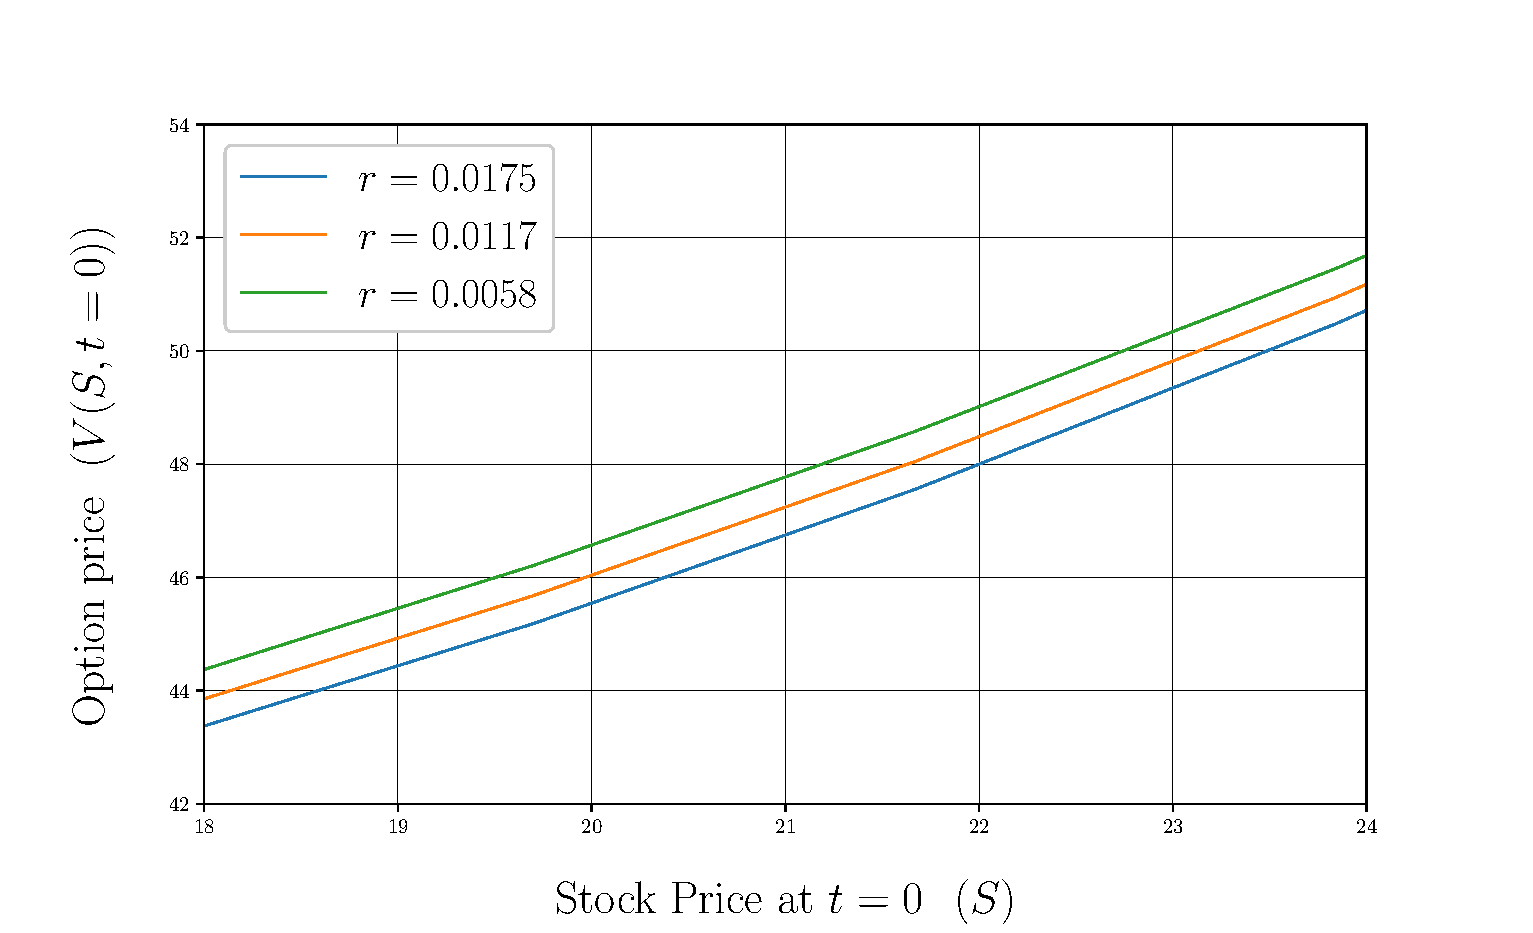
\includegraphics[scale=0.36]{img/Q2/amConvBondValues_incrS_DifferentInterestRatesZoom}
		\captionsetup{width=0.65\linewidth,font=footnotesize}
		\caption{Zoom on $V(S,0)\in [18,24]$.}\label{analysis_different_r_Zoom}
	\end{subfigure}
	\caption{Value of the contract with $r\in\{0.0058,0.0117,0.0175\}$ as $S$ increases.}\label{analysisDifferent_r}
\end{figure}

		\subsection{Value of the contract with an embedded put option when $S_0=17.38$.}
			In this section we are trying to find the most possible accurate value for $V(17.38,0)$ and further obtain in less than one second. To do so, we are going to repeat the same procedure than in Section 1, that is, increase $I$ and $J$ in order to study the convergence rate of Crack Nicolson method in our particular situation, which is \textit{a priori} $\mathcal{O}\left((\Delta S)^2, (\Delta t)^2\right)$. The main difference here is that not only we must try to get $S_0$ within the (vertical) grid points to reduce eventual interpolation errors but also $t_0 = 0.96151$ (within the horizontal axis). 
\begin{table}[h!]\scriptsize
	\setlength{\tabcolsep}{15pt}
	\renewcommand{\arraystretch}{1.2}
	\begin{tabular}{cclll}
		$\texttt{m_I}$ & $\texttt{m_J}$& Without Extrap.&Ratios (\texttt{diffOld/diff}) & One Extrap. (deg.=2)\\ \hline\addlinespace[0.2cm]
		32 	&    16 & 42.7226015285 & &43.398548157933334                  \\
		64 	&    32 & 43.079752062 &5.677829649105139& 43.19880223983333   \\
		128 &   64 & 43.18821969729999 & 3.292692170454403& 43.224375575733326  \\
		256 &   128 & 43.2219325264 & 3.217399375715954& 43.23317013610001  \\
		512 &   256 &  43.230133027600004 &4.111069345372084 &43.23286652800001      \\
		1024 &  512 & 43.2318990171 &4.6435730223934675 & 43.232487680266665 \\
		2048 &  1024 & 43.2327402217 & 2.0993578732129685&43.23302062323333  \\
		4096 &  2048 & 43.233638732399996 & 0.9362210155126094&43.23393823596666   \\
		8192 & 4096 & 43.2338258054 & 4.8029950872996325&43.23388816306667   \\
		16384 & 8192 & 43.2337964887 & 6.381107014103734&43.23378671646666   \\	
	\end{tabular}
	\vspace{0.4cm}
	\captionsetup{width=.5\linewidth}
	\caption{Values when increasing $\texttt{m_I}$ and $\texttt{m_J}$, Lagrange Interpolation of degree $16$ and $S_{max} = 8X$.}\label{table6}
\end{table}
To do so, we must note that there must exist two integers $j^*$ and $i^*$ such that $j^* \texttt{m_dS = S0}$ and $i^* \texttt{m_dt = t_0}$. This implies that $\texttt{m_J} = j^* \texttt{Smax / S0}$ and $\texttt{m_I} = i^* \texttt{T} / t_0$. In our case, $X = S_0$, so we can set $\texttt{Smax = k*X}$ for some integer $k$, and therefore $\texttt{m_J} = \texttt{n * ceil(Smax/S0) = n*k}$, for any integer $\texttt{n}$. We have not such a relation between $\texttt{T}$ and $t_0$, because it's fixed. Therefore, set $\texttt{m_I} =  \texttt{n * ceil(\texttt{T}/t_0)}$, and, although it might not be exactly on the grid, it would not be very far from being on it. Hence, we can try a loop $\texttt{for (int n=nMin; n<=nMax; n*=2)}$ in order to get the Table \ref{table6}.

As we can see in this table, the ratio of the convergence\footnote{We increase $n$ by doubling it each lap. Since the convergence is $\mathcal{O}\left((\Delta S)^2, (\Delta t)^2\right)$, if we double $n$, the value would increase as a ratio of $4$ with respect to the previous difference, i.e., if we take three values $v_m, v_{2m}, v_{4m}$ with $m\equiv 0  \text{ mod } n$,then
$$
	\frac{v_{2n} - v_{n}}{v_{4n} - v_{2n}}\approx 2^2 = 4.
$$} is around $2$, although the monotony is pointly broken. It may be caused by a higher disparity between the new result and the previous one (the greater the denominator, the smaller the result). On the contrary, we get 5 or 6 when the values are similar (opposite~situation). Nevertheless, the ratios are around $4$, so we can explore using Richardson extrapolation ($p=2$) to see whether we can improve our results with less iterations.

Generally speaking, we can see that $V(S_0,0)$ converges to $43.2337\pm10^{-4}$, i.e., we can only ensure three digits of precision (in a reasonable time), i.e., $V(S_0,0)\approx 42.233$. On the other hand, as we can see in Table \ref{table6}, we just need to run our code for $\texttt{(m_I, m_J)} = (128, 64)$ and $\texttt{(m_I, m_J)} = (256, 128)$. 

\vspace{-0.1cm}
\begin{table}[h!]\small
	\setlength{\tabcolsep}{18pt}
	\renewcommand{\arraystretch}{1.15}
	\begin{tabular}{ccll}
		$\texttt{m_I}$ & $\texttt{m_J}$& $V(S_0,0)$ & Time (s)\\ \hline\addlinespace[0.2cm]
		128 &   64 & 43.18821969729999 &  0.0107786  \\
		256 &   128 & 43.2219325264 &  0.039997  \\\addlinespace[0.2cm]\hline\hline\addlinespace[0.1cm]
		\multicolumn{2}{c}{Extrap. Value} & 43.23317013610001 & $9.999 \times 10^{-6}$ \\\addlinespace[0.1cm]\hline\hline
	\end{tabular}
	\vspace{0.4cm}
	\captionsetup{width=.5\linewidth}
	\caption{Obtaining $V(S_0,0)$ with three digits of precision in less than one second.}\label{table7}
\end{table}
\vspace{-0.6cm}
The extrapolated value has been obtain by a simple code which can be found in \texttt{GeneralFunctions.cpp}. Doing that, we obtaing that $V(S_0,0)\approx 42.233$ in 0.05758599 s.


				
	%& APPENDIXES
		%%% SETTING EVERYTHING
		\renewcommand{\thesubsection}{\Alph{subsection}}
		\titleformat{\subsection}
		{\normalfont\large\bfseries}{Appendix \thesubsection.}{0.5em}{}
		\titleformat{\subsubsection}
		{\normalfont\normalsize}{Appendix \thesubsubsection}{1em}{}
	\newpage
	\setcounter{secnumdepth}{0}
	\section{Appendices}
	%%% COUNTERS
		\setcounter{secnumdepth}{4}
		\setcounter{tocdepth}{6}
		\setcounter{subsection}{0}
		%%% THE APPENDIXES
		%& APPENDIX I: SOLUTION FOR THE ODE FOR C
		\subsection{Boundary conditions: Solving the ODE to obtain $B(t)$ for large $S$}\label{app_ODE_C}
			In this Appendix we provide the derivation of the solution of (\ref{C_ode}) by solving the integral written in~(\ref{C_ode_sol}):
$$
\begin{aligned}
	C(t) 	&= B_T + \int_t^T \exp{r(T-s)}f(s)\d s\\
	&= B_T + \int_t^T \exp{r(T-s)}\left[\kappa X A(s) + C\exp{-\alpha s}\right]\d s\\
	&= B_T + \int_t^T \left[\kappa X R \exp{- (\kappa + r) (T-s)} \exp{r(T-s)} + C\exp{-(r+\alpha)s+rT}\right]\d s\\
	&= B_T + \int_t^T \left[\kappa X R \exp{-\kappa (T-s)} + C\exp{-(r+\alpha)s +rT}\right]\d s\\
	&= B_T + {X R \exp{-\kappa T}}  \left[\exp{\kappa T} - \exp{\kappa t}\right] - \frac{C}{r+\alpha}\exp{rT}\left[\exp{-(r+\alpha)T}-\exp{-(r+\alpha)t}\right]\\
	&= B_T + {X R}  \left[1 -  \exp{-\kappa(T-t)}\right]- \frac{C}{r+\alpha}\exp{rT}\left[\exp{-(r+\alpha)T}-\exp{-(r+\alpha)t}\right] .
\end{aligned}
$$
			\newpage
		%& APPENDIX II: VALUE FUNCTION WHEN S=0
		\subsection{Boundary conditions: Value function when $S=0$}\label{app_bound_V_S0}
			Now, we will find the solution for the PDE given in (\ref{pde_S0}), i.e., 
\begin{equation}
	\partial_t V + \kappa \theta(t) \partial_S V - r V + C \exp{-\alpha t} = 0,
\end{equation}
with the boundary condition given by 
\begin{equation}
	V(S=0,T) = F.
\end{equation}

We are going to use the method of characteristic, because it is a first order differential equation. To do so, note that (\ref{pde_S0}) can be written as
\begin{equation}
	a \partial_t V + b(t) \partial_S V + c V = f(t),
\end{equation}
where $a \equiv 1$, $b(t) = \kappa \theta(t)$, $c\equiv -r$ and $f(t) = -Ce^{-\alpha t}$. Hence, the characteristic equation is
\begin{equation}\label{char_eq}
	S'(t) = \kappa  \theta(t).
\end{equation}

Note that $\theta(t) = \frac{1}{\mu}\theta'(t)$, which implies that (\ref{char_eq}) is solved by
\begin{equation}
	S(t) = \frac{\kappa}{\mu} \theta(t) + \text{cte},
\end{equation}
i.e., it describes a whole family of solutions given by the integral curves defined by the following equation
\begin{equation}\label{integral_curves}
	B(S,t) = S - \frac{\kappa}{\mu} \theta(t) \equiv \text{cte}.
\end{equation}
By choosing $A(t) = t$, we obtain that the Jacobian 
\begin{equation}
	J = \partial_S B(S, t)  = 1 \not = 0,
\end{equation}
as required. Hence, we can write $V$ as $V(S,t) = \omega(A(t), B(S,t))$, from which, by the chain rule, we obtain
\begin{equation}\label{chain_rule}
	\begin{aligned}
		\partial_t V& = \partial_A \omega \ A'(t) + \partial_B \omega \ \partial_t  B(S,t)\\
		\partial_S V& = \partial_B \omega \ \partial_S B(S,t)
	\end{aligned}
\end{equation}
Now calculate the derivatives
\begin{equation}
	A'(t) = 1; \doublequad  \partial_tB (S,t) = -\kappa \theta(t); \doublequad \partial_SB(S,t) = 1,
\end{equation}
and substitute them into (\ref{chain_rule}) to obtain
\begin{equation}
	\begin{aligned}
		\partial_t V& = \partial_A \omega +  -\kappa\theta(t)\partial_B \omega \ \\
		\partial_S V& = \partial_B \omega, 
	\end{aligned}
\end{equation}
and substitue it into (\ref{pde_S0}) to obtain
$$
\begin{aligned}
	\partial_A \omega   -\kappa\theta(t)\partial_B \omega + \kappa \theta(t) \partial_B \omega - r \omega + C \exp{-\alpha A} &= 0,	\\
	\partial_A \omega  - r \omega + C \exp{-\alpha A} &= 0,\\
	\partial_A \omega \exp{-rA}  - r \omega \exp{-rA} + C \exp{-(\alpha+r) A} &= 0,\\
	\partial_A\left(\omega \exp{-rA}\right) = -C \exp{-(\alpha+r)A},
\end{aligned}
$$
and therefore
\begin{equation}
	V(S,t) =  \frac{C}{r+\alpha}\exp{-\alpha t} + M \ \exp{rt},
\end{equation} 
where $M$ must be derived from initial conditions:
\begin{equation}
	\begin{aligned}
		V(S,t) &=  \frac{C}{r+\alpha}\exp{-\alpha t} + F \exp{-r(T-t)} - \frac{C}{r+\alpha}\exp{-(\alpha+r) T + rt}\\
		&=\frac{C}{r+\alpha}\exp{-\alpha t} + F \exp{-r(T-t)} - \frac{C}{r+\alpha}\exp{-\alpha T -r(T-t)}\\
	\end{aligned}
\end{equation}

Finally,
\begin{equation}
	V(S=0,t) =  F \exp{-r(T-t)} + \frac{C}{r+\alpha} \exp{-\alpha T}\left( \exp{\alpha (T-t)} -\exp{-r(T-t)} \right).
\end{equation}
			\newpage
		%& APPENDIX III: DERIVATION OF THE COEFFICIENT FUNCTIONS
		\subsection{Approximation of the coefficients for the Crank-Nicolson method}\label{app_coeff_CrankNic}
			We are asked to find a numerical solution for the following PDE
\begin{equation}\label{PDE}
	\partial_t V + \frac{1}{2}\sigma^2 S^{2\beta} \partial_{SS}V + \kappa(\theta(t) - S)\partial_S V - rV + C \exp{-\alpha t} = 0.
\end{equation}

Here we present a derivation of the numerical approximation formul\ae. To do so, firstly recall the formula for an approximation for $V$
\begin{equation}
		V \approx \frac{1}{2}\left(V_{i,j} + V_{i+1,j}\right),
\end{equation}
and the formul\ae for the approximations of the partial derivatives: firstly with respect to $t$
\begin{equation}\label{partial_wrt_t}
	\partial_t V \approx \frac{V_{i+1,j} - V_{i,j}}{\Delta t};
\end{equation}
and secondly, with respect to $S$, the first derivative
\begin{equation}\label{first_wrt_S}
	\partial_S V 	\approx \frac{1}{4\Delta S}\left(V_{i,j+1} - V_{i,j-1} + V_{i+1,j+1} - V_{i+1,j-1}\right),
\end{equation}
and the second derivative
\begin{equation}\label{second_wrt_S}
	\partial_{SS} V	\approx \frac{1}{2\Delta S^2}\left(V_{i,j+1} - 2V_{i,j } + V_{i,j-1}+ V_{i+1,j+1}-2V_{i+1,j} + V_{i+1,j-1}\right)
\end{equation}
By substituting there approximation into (\ref{PDE}), then
$$
	\begin{aligned}
		0 	&= \frac{V_{i+1,j} - V_{i,j}}{\Delta t} \\
			&+ \frac{1}{2}\sigma^2 S^{2\beta} \frac{1}{2\Delta S^2}\left(V_{i,j+1} - 2V_{i,j } + V_{i,j-1}+ V_{i+1,j+1}-2V_{i+1,j} + V_{i+1,j-1}\right) \\
			&+ \kappa(\theta(\Delta t) - S)\frac{1}{4\Delta S}\left(V_{i,j+1} - V_{i,j-1} + V_{i+1,j+1} - V_{i+1,j-1}\right) \\
			&- r\frac{1}{2}\left(V_{i,j} + V_{i+1,j}\right) + C \exp{-\alpha \Delta t}.
	\end{aligned}
$$
Rearranging terms
\begin{align*}
		&\phantom{+} \left(-\frac{1}{4}\sigma^2j^{2\beta}S^{2(\beta -1)}+ \frac{\kappa}{4}\left[\frac{\theta(\Delta t)}{\Delta S} - j\right]\right)V_{i,j-1} \\
		&+ \left(\frac{1}{\Delta t} + \frac{r}{2} + \frac{1}{2}\sigma^2 \left(\Delta S\right)^{2(\beta - 1)} \right)V_{i,j} \\
		&+ \left( -\frac{1}{4}\sigma^2j^{2\beta}S^{2(\beta -1)} - \frac{\kappa}{4}\left[\frac{\theta(\Delta t)}{\Delta S} - j\right]\right) V_{i, j+1}\\
		&= \left(\frac{1}{4}\sigma^2 j^{2\beta}S^{2(\beta - 1)} - \frac{\kappa}{4}\left[\frac{\theta(\Delta t)}{\Delta S} - j\right]\right)V_{i+1,j-1}\\
		&+ \left(\frac{1}{\Delta t } - \frac{1}{2}\sigma^2 j^2S^{2(\beta - 1)}  - \frac{r}{2}\right)V_{i+1,j}\\
		&+ \left(\frac{1}{4}\sigma^2 j^{2\beta}S^{2(\beta - 1)}+ \frac{\kappa}{4}\left[\frac{\theta(\Delta t)}{\Delta S} - j\right]\right)V_{i+1,j+1} + C \exp{-\alpha \Delta t}.
\end{align*}

and hence
\begin{equation}
	\begin{aligned}
		a(j) &= -\frac{1}{4}\sigma^2j^{2\beta}(\Delta S)^{2(\beta -1) }+ \frac{\kappa}{4}\left[\frac{\theta(\Delta t)}{\Delta S} - j\right] \\
		b(j) &= \frac{1}{\Delta t} + \frac{r}{2} + \frac{1}{2}\sigma^2 j^{2\beta}(\Delta S)^{2(\beta -1) }\\
		c(j) &=  -\frac{1}{4}\sigma^2j^{2\beta}(\Delta S)^{2(\beta -1) } - \frac{\kappa}{4}\left[\frac{\theta(\Delta t)}{\Delta S} - j\right]\\
		d(i,j)&=\left(\frac{1}{4}\sigma^2 j^{2\beta}(\Delta S)^{2(\beta -1) } - \frac{\kappa}{4}\left[\frac{\theta(\Delta t)}{\Delta S} - j\right]\right)V_{i+1,j-1}\\
		&+ \left(\frac{1}{\Delta t } - \frac{1}{2}\sigma^2 j^{2\beta}(\Delta S)^{2(\beta -1) }  - \frac{r}{2}\right)V_{i+1,j}\\
		&+ \left(\frac{1}{4}\sigma^2 j^{2\beta}(\Delta S)^{2(\beta -1) }+ \frac{\kappa}{4}\left[\frac{\theta(\Delta t)}{\Delta S} - j\right]\right)V_{i+1,j+1} + C \exp{-\alpha \Delta t}.
	\end{aligned}
\end{equation}


			\newpage
		%& APPENDIX V: CODE
		\subsection{Code}	\label{app_code}
			We have organised our code in two main folders called \texttt{finDif} and \texttt{aux}. The first folder contains the main files of the Crank Nicolson method, \texttt{CrankNicolson.cpp} and \texttt{CrankNicolson.h} and two more files, \texttt{taks} and \texttt{aux}. The former contains the especific classes for solving both tasks, whist the latter contains auxiliar functions for the Crank Nicolson Method such that the set up of the Convertible Bond, \texttt{ConvertibleBonds.cpp} and\texttt{ConvertibleBonds.h} or functions for constructing the grid, \texttt{GridConstructos.cpp} and \texttt{GridConstructor.h}.

Within the \texttt{aux} function we can find files for printing macros and other general functions.

\subsubsection{\texttt{main.cpp}}
Here we provide the \texttt{main.cpp}. Most of functions are commented. To print something one just has to remove the \texttt{//}. 
\begin{lstlisting}
	#include <cmath>
	#include <vector>
	#include <algorithm>
	
	#include <iostream>
	#include <fstream>
	// For this task
	#include "CrankNicolson.h"
	#include "ConvertibleBonds.h"
	#include "Q1.h"
	#include "Q2.h"
	// General
	#include "GeneralFunctions.h"
	// To calculate the time
	#include <chrono>
	#define  CHRONO   std::chrono
	#define  SET_TIME CHRONO::system_clock::now()
	#define  DURATION CHRONO::duration
	#define  MILLI    std::milli
	
	#define NEXT_CASE cout << "#######" << endl;
	
	using namespace std;
	/* Template code for the Crank Nicolson Finite Difference
	*/
	int main(){
		cout.precision(15);
		// PARAMETERS
		double T = 3., F = 35., R = 2, r = 0.0117, kappa = 0.0833333333333, mu = 0.0053, X = 17.38, C = 0.205, alpha = 0.02, beta = 0.808, sigma = 0.66;
		double Smax = 250;
		double I = 500;
		double J = 500;
		ofstream output;
		Q1 q1(T, F, R, r, kappa, mu, X, C, alpha, beta, sigma, 1000, I, J);
		Q2 q2(T, F, R, r, kappa, mu, X, C, alpha, beta, sigma, 1000, I, J);
		/*
		TASK 1
		*/
		//    CONV_BONDS convBond(T, F, R, r, kappa, mu, X, C, alpha, beta, sigma, Smax, J, I);
		//    cout << (F - convBond.B(0)) / convBond.A(0) << endl;
		
		///
		/// FIXING BETA AND MOVING SIGMA
		///
		// vector <double> sigmas = {0, 0.381, 0.66, 0.802, 0.962, 1};
		// q1.variousSigmas(sigmas, THOMAS);
		
		///
		/// FIXING SIGMA AND MOVING BETA
		///
		// vector <double> betas = {0.892};
		// q1.variousBetas(betas, THOMAS);
		
		///
		/// FIXING SIGMA AND AND BETA AND MOVING KAPPA
		///
		// vector <double> kappas = {0, 0.02, 0.0833, 0.2, 0.5, 1};
		// q1.variousKappas(kappas, THOMAS);
		
		///
		/// INCREASING IMAX AND JMAX (SQUARE) AND FIXING SMAX
		///
		//  q1.variousV_fixedS0(17.38, 2, 2, 20000, 16, 8.);
		//  vector<double> v = {42.0495722630, 42.0495647830, 42.0495620065};
		//  q1.V_fixedS0(17.38, 16, 8., 952, 952);
		//  q1.V_fixedS0(17.38, 16, 8., 9216, 9216);
		//  AUX::extrap(v[1], v[2], 2);
		
		/*
		TASK 2
		*/
		//    q1.increasingS(500, 500, 300, 1.05);
		//    q2.increasingS(100, 100, 200, 1.05);
		//    q2.increasingS(200, 200, 200, 1.05);
		//    vector<double> rs = {0.00585, 0.0117, 0.01755};
		//    q2.variousInterestRates(rs, 300, 300, 200);
		//    q2.variousV_fixedS0(17.38, 0.96151, 2, 2, 80000, 16, 8.);
		//    q2.V_fixedS0(17.38, 0.96151, 16, 8., 128, 64);
		//    q2.V_fixedS0(17.38, 0.96151, 16, 8., 256, 128);
		//    AUX::extrap(43.18821969729999, 43.2219325264, 2);
		return 0;
	}
\end{lstlisting}

\subsubsection{\texttt{finDif} folder}

\begin{lstlisting}
	//
	//  CrankNicolson.h
	//  assignment2_codes
	//
	//  Created on 28/4/21.
	//
	
	#include <vector>
	#include <iostream>
	#include <fstream>
	using namespace std;
	
	#define CN  CCrankNicolson
	#define LU      1
	#define SOR     2
	#define THOMAS  3
	
	#define PSOR                1
	#define POLICY_ITERATION    2
	#define PENALTY             3
	
	#define EUROPEAN false
	#define AMERICAN true
	
	#define SAVE        true
	#define DONT_SAVE   false
	
	class CCrankNicolson
	{
		public:
		CCrankNicolson(double T, double F, double R, double r, double kappa, double mu, double X, double C, double alpha, double beta, double sigma, double S0, double Smax, long I, long J);
		// Main functions
		void eurConvertibleBond(ofstream *output, int method = 0, int degree = 2, double tol = 1.e-2, double omega = 1.2);
		void amConvertibleBond_penalty(ofstream *output, int degree=2, bool saveData = true, double tol = 1.e-6);
		// Get Option Value
		inline double GetV() {return m_optionValue;};
		private:
		// Useful Functions
		double approxPrice(vector<double> &v, vector<double> &s);
		vector<double> thomasSolve(const vector<double> &a,const vector<double> &b_,const vector<double> &c, vector<double> &d);
		// PARAMETERS
		double m_T;
		double m_F;
		double m_R;
		double m_r;
		double m_kappa;
		double m_mu;
		double m_X;
		double m_C;
		double m_alpha;
		double m_beta;
		double m_sigma;
		// AMERICAN PARAMETERS
		double m_P;
		double m_rho;
		double m_iterMax;
		double m_t0;
		// AUXILIAR PARAMETERS
		double m_kappar;
		double m_alphar;
		// Local Variables (dS, dt)
		double m_S0;
		double m_Smax;
		double m_dS;
		double m_dt;
		// Grid Parameters
		long   m_J;
		long   m_I;
		int    m_jStar;
		// Option Value
		double m_optionValue;
	};
\end{lstlistings}

\begin{lstlisting}
	//
	//  CrankNicolson.cpp
	//  assignment2_codes
	//
	//  Created  on 28/4/21.
	//
	
	/// Header of the explicit difference method
	#include "CrankNicolson.h"
	
	/// Header with convertible bonds functions
	#include "ConvertibleBonds.h"
	
	/// Header with some important and useful functions
	#include "GeneralFunctions.h"
	
	/// Header with payoff functions of several options
	#include "PayoffFunctions.h"
	
	/// Header for constructing the grid of the explicit difference method
	#include "GridConstructor.h"
	
	/// Header for printing data
	#include "PrintMacros.h"
	
	// To calculate the time
	#include <chrono>
	#define  CHRONO   std::chrono
	#define  SET_TIME CHRONO::system_clock::now()
	#define  DURATION CHRONO::duration
	#define  MILLI    std::milli
	
	/// Important libraries
	#include <cmath>
	#include <algorithm>
	#include <vector>
	#include <iostream>
	#include <fstream>
	using namespace std;
	
	/// First declare the parameters for the problem, local grid and variables and the vectors required
	/// In option pricing problems, we must for S over the semi infinite domain, therefore numerically we need to choose an appropiate Smax
	/// The first five parameters are intrinsice option parameters, whilst the last three ones are those appropriate parameters for the method.
	
	CN::CCrankNicolson(double T, double F, double R, double r, double kappa, double mu, double X, double C, double alpha, double beta, double sigma, double S0, double Smax, long I, long J){
		m_T         = T;
		m_F         = F;
		m_R         = R;
		m_r         = r;
		m_kappa     = kappa;
		m_mu        = mu;
		m_X         = X;
		m_C         = C;
		m_alpha     = alpha;
		m_beta      = beta;
		m_sigma     = sigma;
		m_kappar    = kappa + r;
		m_alphar    = alpha + r;
		m_S0        = S0;
		m_Smax      = Smax;
		m_J         = J;
		m_I         = I;
		m_dS       = m_Smax / J;
		m_dt        = m_T / I;
		m_jStar     = m_S0/m_dS;
	}
	void
	CN::eurConvertibleBond(ofstream *output, int method, int degree, double tol, double omega)
	{
		// CONVERTIBLE BONDS LIBRARY
		CONV_BONDS convBonds(m_T, m_F, m_R, m_r, m_kappa, m_mu, m_X, m_C, m_alpha, m_beta, m_sigma, m_Smax, m_I, m_J);
		//
		vector <double> vOld(m_J+1), vNew(m_J+1);
		// Setup and initialise the stock price
		vector <double> S = GRID::setupStockPrices(m_dS, m_J);
		// Setup and initialise the final conditions on the option price
		for (int j=0; j<=m_J; j++)
		{
			vOld[j] = PAYOFF::convBond(S[j], m_R, m_F);
			vNew[j] = PAYOFF::convBond(S[j], m_R, m_F);
			// PRINT_5DATA_LINE(m_I, j, S[j], vNew[j], vOld[j])
		}
		// start looping through time levels
		for(long i=m_I-1; i>=0; i--)
		{
			double t        = i * m_dt;
			double approx_t = (i + 0.5) * m_dt;
			/// BOUNDARY CONDITIONS
			// Declare vectors for matrix equations
			vector<double> a = {0.}, b = {1.}, c = {0.}, d = {convBonds.V_S0(approx_t)};
			// LU method
			vector<double> beta = {b[0]}, D = {d[0]};
			
			/// SET UP MATRIX EQUATIONS
			// PRINT_4DATA_LINE("a", "b", "c", "d")
			// PRINT_4DATA_LINE(a[0], b[0],c[0], d[0])
			for(int j=1;j< m_J;j++)
			{
				a.push_back(convBonds.aFunc(i, j));
				b.push_back(convBonds.bFunc(i, j));
				c.push_back(convBonds.cFunc(i, j));
				d.push_back(convBonds.dFunc(i, j, vOld));
				// LU method
				if (method == LU)
				{
					beta.push_back(convBonds.betaFunc(approx_t, j, beta[j-1]));
					D.push_back(convBonds.DFunc(approx_t, j, beta[j-1], d[j], D[j-1]));
				}
			}
			// Boundary conditions at S = Smax
			a.push_back(0.);
			b.push_back(1.);
			c.push_back(0.);
			d.push_back(convBonds.V_Smax(m_Smax,approx_t));
			
			// EUROPEAN OPTIONS
			// SOLVE WITH LU METHOD
			if (method == LU)
			{
				beta.push_back(convBonds.betaFunc(i, m_J, beta[m_J-1]));
				D.push_back(convBonds.DFunc(i, m_J, beta[m_J-1], d[m_J], D[m_J-1]));
				// Solve matrix equations with LU method
				vNew[0] = m_X;
				vNew[m_J] = D[m_J] / beta[m_J];
				for (long j=m_J-1; j >=0; j--)
				vNew[j] = convBonds.prevV(t, j, beta, D, vNew);
			}
			// SOLVE WITH SOR METHOD
			if (method == SOR)
			{
				// Solve matrix equations with SOR
				long y, sor, iterMax = 10000;
				for (sor = 0; sor < iterMax; sor++)
				{
					// SOR equations in here
					// j = 0
					{
						y = (d[0] - c[0] * vNew[1]) / b[0];
						vNew[0] = vNew[0] + omega * (y-vNew[0]);
					}
					// 0 < j < jMax
					for(long j=1; j<m_J; j++)
					{
						y = (d[j] - a[j] * vNew[j-1] - c[j]*vNew[j+1]) / b[j];
						vNew[j] = vNew[j] + omega * (y-vNew[j]);
					}
					// j = jMax
					{
						y = (d[m_J] - a[m_J] * vNew[m_J-1]) / b[m_J];
						vNew[m_J] = vNew[m_J] + omega * (y-vNew[m_J]);
					}
					// Calculate residual
					double error=0.;
					error += fabs(d[0] - b[0] * vNew[0] - c[0] * vNew[1]);
					for(long j=1; j<m_J;j++)
					error += fabs(d[j] - a[j]*vNew[j-1] - b[j]*vNew[j] - c[j]*vNew[j+1]);
					error += fabs(d[m_J] - a[m_J]*vNew[m_J-1] - b[m_J]*vNew[m_J]);
					// Check for convergence and exit loop if converged
					if(error < tol)
					break;
				}
				if(sor==iterMax)
				PRINT_DATA_LINE("NOT CONVERGED");
			}
			// SOLVE WITH THOMAS SOLVER ALGORITHM
			if (method == THOMAS)
			vNew = thomasSolve(a, b, c, d);
			// Set old=new
			vOld = vNew;
		}
		// Finish looping through time levels
		// output the estimated option price
		double optionValue = GRID::lagrangeInterpolation(vNew, S, m_S0, degree);//approxPrice(vNew, S);
		// output the estimated option price
		double asympV = m_S0*convBonds.A(0) + convBonds.B(0);
		DATA_LINE(output, m_F, m_I, m_J, m_S0, optionValue, asympV);
		PRINT_DATA_LINE(m_F, m_I, m_J, m_S0, optionValue, asympV);
		
	}
	
	void
	CN::amConvertibleBond_penalty(ofstream *output, int degree, bool saveData, double tol)
	{
		
		m_P = 38.;
		m_t0 = 0.96151;
		m_iterMax = 10000;
		m_rho = 1e8;
		
		// CONVERTIBLE BONDS LIBRARY
		CONV_BONDS convBonds(m_T, m_F, m_R, m_r, m_kappa, m_mu, m_X, m_C, m_alpha, m_beta, m_sigma, m_Smax, m_I, m_J);
		//
		vector <double> vOld(m_J+1), vNew(m_J+1);
		// Setup and initialise the stock price
		vector <double> S = GRID::setupStockPrices(m_dS, m_J);
		// Setup and initialise the final conditions on the option price
		for (long j=0; j<=m_J; j++)
		{
			vOld[j] = PAYOFF::convBond(S[j], m_R, m_F);
			vNew[j] = PAYOFF::convBond(S[j], m_R, m_F);
			// PRINT_5DATA_LINE(m_I, j, S[j], vNew[j], vOld[j])
		}
		// start looping through time levels
		for(long i=m_I-1; i>=0; i--)
		{
			double t        = i*m_dt;
			double approx_t = (i + 0.5) * m_dt;
			/// BOUNDARY CONDITIONS
			// Declare vectors for matrix equations
			vector<double> a = {0.}, b = {1.}, c = {0.}, d;
			if (approx_t <= m_t0)
			d = {max(m_P,convBonds.V_S0(approx_t))};
			else
			d = {convBonds.V_S0(approx_t)};
			/// SET UP MATRIX EQUATIONS
			for(int j=1;j< m_J;j++)
			{
				a.push_back(convBonds.aFunc(i, j));
				b.push_back(convBonds.bFunc(i, j));
				c.push_back(convBonds.cFunc(i, j));
				d.push_back(convBonds.dFunc(i, j, vOld));
			}
			// Boundary conditions at S = Smax
			a.push_back(0.);
			b.push_back(1.);
			c.push_back(0.);
			// d.push_back(convBonds.V_Smax(m_Smax,approx_t));
			d.push_back(m_R*m_Smax);
			// Temporal restriction
			int penaltyIt;
			for (int penaltyIt=0; penaltyIt < m_iterMax; penaltyIt++)
			{
				// Create new vectors containing a copy of the FD approx
				vector<double> aHat(a), bHat(b), cHat(c), dHat(d);
				// Apply penalty here to finite difference scheme
				for (int j=1; j<m_J; j++)
				{
					// If current value suggesta apply penalty, adjust matrix equations
					if(vNew[j] < m_R*S[j])
					{
						bHat[j] = b[j] + m_rho;
						dHat[j] = d[j] + m_rho*(m_R*S[j]);
					}
					if( approx_t < m_t0 && vNew[j] < m_P)
					{
						bHat[j] = bHat[j] + m_rho;
						dHat[j] = dHat[j] + m_rho*m_P;
					}
					
				}
				// Solve with thomas Method
				vector <double> y = thomasSolve(aHat, bHat, cHat, dHat);
				// y now contains next guess at solution
				// Check for differences between vNew and y
				double error = 0.;
				for (int j=0; j<= m_J; j++)
				error += (vNew[j] - y[j])*(vNew[j] - y[j]);
				// Update Value of vNew
				vNew = y;
				// make an exit condition when solution is converged
				if (error < tol * tol)
				break;
			}
			if(penaltyIt >= m_iterMax)
			{
				PRINT_DATA_LINE("Error NOT converging within required iterations");
				throw;
			}
			vOld=vNew;
		} // Ending temporal loop
		
		// Finish looping through time levels
		// output the estimated option price
		m_optionValue = GRID::lagrangeInterpolation(vNew, S, m_S0, degree);//approxPrice(vNew, S);
		// output the estimated option price
		double asympV = m_S0*convBonds.A(0) + convBonds.B(0);
		if (saveData == SAVE)
		{
			DATA_LINE(output, m_F, m_I, m_J, m_S0, m_optionValue, asympV);
		}
		PRINT_DATA_LINE(m_F, m_I, m_J, m_S0, m_optionValue, asympV);
	}
	
	
	// USEFUL FUNCTIONS
	double
	CN::approxPrice(vector<double> &v, vector<double> &s)
	{
		vector<double> p1 = {s[m_jStar], v[m_jStar]};
		vector<double> p2 = {s[m_jStar+1], v[m_jStar+1]};
		return AUX::lagInterp(m_S0, p1, p2);
	}
	
	vector<double>
	CN::thomasSolve(const vector<double> &a,const vector<double> &b_,const vector<double> &c, vector<double> &d)
	{
		auto n=a.size();
		std::vector<double> b(n),temp(n);
		// initial first value of b
		b[0]=b_[0];
		for(auto j=1;j<n;j++)
		{
			b[j]=b_[j]-c[j-1]*a[j]/b[j-1];
			d[j]=d[j]-d[j-1]*a[j]/b[j-1];
		}
		// calculate solution
		temp[n-1]=d[n-1]/b[n-1];
		for(int j=n-2; j>=0; j--)
		temp[j]=(d[j]-c[j]*temp[j+1])/b[j];
		return temp;
	}
	
	//if (method == PSOR){
		//    // Solve matrix equations with SOR
		//    int y, sor, iterMax = 10000;
		//    for (sor = 0; sor < iterMax; sor++)
		//    {
			//        // SOR equations in here
			//        // j = 0
			//        {
				//          y = (d[0] - c[0] * vNew[1]) / b[0];
				//          vNew[0] = max(vNew[0] + omega * (y-vNew[0]), m_P);
				//        }
			//        // 0 < j < jMax
			//        for(int j=1; j<m_J; j++)
			//        {
				//          y = (d[j] - a[j] * vNew[j-1] - c[j]*vNew[j+1]) / b[j];
				//          vNew[j] = max(vNew[j] + omega * (y-vNew[j]), m_P);
				//        }
			//        // j = jMax
			//        {
				//          y = (d[m_J] - a[m_J] * vNew[m_J-1]) / b[m_J];
				//          vNew[m_J] = max(vNew[m_J] + omega * (y-vNew[m_J]), m_P);
				//        }
			//        // Calculate residual
			//        double error=0.;
			//        error += fabs(d[0] - b[0] * vNew[0] - c[0] * vNew[1]);
			//        for(int j=1; j<m_J;j++)
			//          error += fabs(d[j] - a[j]*vNew[j-1] - b[j]*vNew[j] - c[j]*vNew[j+1]);
			//        error += fabs(d[m_J] - a[m_J]*vNew[m_J-1] - b[m_J]*vNew[m_J]);
			//        // Check for convergence and exit loop if converged
			//        if(error < tol)
			//          break;
			//    }
		//}
\end{lstlisting}

\begin{lstlisting}
	//
	//  PayoffFunctions.hpp
	//  ComputationalFinance
	//
	//  Created on 14/4/21.
	//
	
	#define  PAYOFF CPayoffFunctions
	
	class CPayoffFunctions{
		public:
		static double callOption(double stock_price, double strike_price);
		static double putOption(double stock_price, double strike_price);
		static double convBond(double stock_price, double R, double F);
	};
\end{lstlisting}
\begin{lstlisting}
	//
	//  PayoffFunctions.cpp
	//  ComputationalFinance
	//
	//  Created on 14/4/21.
	//
	
	#include "PayoffFunctions.h"
	#include "GeneralFunctions.h"
	
	// CALL OPTION PAYOFF
	double
	PAYOFF::callOption(double stock_price, double strike_price){
		return AUX::maxFunc(stock_price - strike_price, 0.);
	}
	
	// PUT OPTION PAYOFF
	double
	PAYOFF::putOption(double stock_price, double strike_price){
		return AUX::maxFunc(strike_price - stock_price, 0.);
	}
	
	// CONVERTIBLE BOND
	double
	PAYOFF::convBond(double stock_price, double R, double F)
	{
		return AUX::maxFunc(F, R * stock_price);
	}	
\end{lstlisting}

\begin{lstlisting}
	//
	//  ConvertibleBonds.hpp
	//  assignment2_codes
	//
	//  Created on 28/4/21.
	//
	
	#define CONV_BONDS CConvertibleBonds
	
	#include <vector>
	#include <iostream>
	#include <fstream>
	using namespace std;
	
	class CConvertibleBonds
	{
		public:
		CConvertibleBonds(double T, double F, double R, double r, double kappa, double mu, double X, double C, double alpha, double beta, double sigma, double Smax, long I, long J);
		
		double V_Smax(double S, double t);
		double V_S0(double t);
		// AUXILIAR FUNCTIONS
		double A(double t);
		double B(double t);
		// COEFFICIENTS FOR THE PDE
		double aFunc(long i, long j);
		double bFunc(long i, long j);
		double cFunc(long i, long j);
		double dFunc(long i, long j, vector<double> &v);
		double theta(double t);
		// LU coefficients
		double betaFunc(long i, long j, double prevBeta);
		double DFunc(long i, long j, double prevBeta, double d, double prevD);
		double prevV(long i, long j, vector<double>& beta, vector<double>& D, vector<double>& V);
		private:
		// PARAMETERS
		double m_T;
		double m_F;
		double m_R;
		double m_r;
		double m_kappa;
		double m_mu;
		double m_X;
		double m_C;
		double m_alpha;
		double m_beta;
		double m_sigma;
		// PDE PARAMETERS
		double m_Smax;
		double m_J;
		double m_I;
		double m_dS;
		double m_dt;
		// AUXILIAR PARAMETERS
		double m_kappar;
		double m_alphar;
		
	};
\end{lstlisting}

\begin{lstlisting}
	//
	//  ConvertibleBonds.cpp
	//  assignment2_codes
	//
	//  Created on 28/4/21.
	//
	
	#include "ConvertibleBonds.h"
	#include <cmath>
	#include <algorithm>
	#include <vector>
	#include <iostream>
	#include <fstream>
	using namespace std;
	
	CONV_BONDS::CConvertibleBonds(double T, double F, double R, double r, double kappa, double mu, double X, double C, double alpha, double beta, double sigma, double Smax, long I, long J)
	{
		m_T         = T;
		m_F         = F;
		m_R         = R;
		m_r         = r;
		m_kappa     = kappa;
		m_mu        = mu;
		m_X         = X;
		m_C         = C;
		m_alpha     = alpha;
		m_beta      = beta;
		m_sigma     = sigma;
		m_kappar    = kappa + r;
		m_alphar    = alpha + r;
		m_Smax      = Smax;
		m_J         = J;
		m_dS        = m_Smax / m_J;
		m_I         = I;
		m_dt        = m_T / m_I;
	}
	
	double
	CONV_BONDS::A(double t)
	{
		return m_R * exp(-m_kappar * (m_T - t));
	}
	
	double
	CONV_BONDS::B(double t)
	{
		double X_term = 2. * m_X * m_R * exp( - (m_r + 0.5 * m_kappa) * (m_T - t) ) * sinh( 0.5 * m_kappa * (m_T -t) );
		double C_term = - m_C / m_alphar * exp(m_r * t) * ( exp(-m_alphar * m_T) - exp(-m_alphar * t));
		return X_term + C_term;
	}
	
	// GENERAL VALUE FUNCTION
	double
	CONV_BONDS::V_Smax(double S, double t)
	{
		return S * A(t) + B(t);
	}
	
	// VALUE FUNCTION WHEN S = 0
	double
	CONV_BONDS::V_S0(double t)
	{
		double F_term = m_F * exp( -m_r * (m_T - t) );
		double C_term = m_C / ( m_r + m_alpha ) * exp( -m_alpha * m_T ) * ( exp(m_alpha * (m_T - t)) - exp(-m_r * (m_T - t)) );
		return F_term + C_term;
	}
	
	// PDE COEFFICIENTS
	double
	CONV_BONDS::aFunc(long i, long j)
	{
		double first_term, second_term;
		double approx_t     = (i + 0.5) * m_dt;
		first_term   = -0.25 * pow(m_sigma, 2.) * pow(j, 2.* m_beta) * pow(m_dS, 2*(m_beta-1));
		second_term  =  0.25 * m_kappa * (theta(approx_t) / m_dS - j);
		return first_term + second_term;
	}
	
	double
	CONV_BONDS::bFunc(long i, long j)
	{
		double long_term = 0.5 * pow(m_sigma, 2.) * pow(j, 2. * m_beta) * pow(m_dS, 2. * (m_beta - 1.));
		return 1. / m_dt + 0.5 * m_r  + long_term;
	}
	
	double
	CONV_BONDS::cFunc(long i, long j)
	{
		double first_term, second_term;
		double approx_t     = (i + 0.5) * m_dt;
		first_term   = -0.25 * pow(m_sigma, 2.) * pow(j, 2.*m_beta) * pow(m_dS, 2. * (m_beta-1.));
		second_term  = -0.25 * m_kappa * (theta(approx_t) / m_dS - j);
		return first_term + second_term;
	}
	
	double
	CONV_BONDS::dFunc(long i, long j, vector<double> &v)
	{
		double approx_t = (i + 0.5) * m_dt;
		double a = aFunc(i, j);
		double b = bFunc(i, j);
		double c = cFunc(i, j);
		double d = - (a * v[j-1] + (b - 2. / m_dt) * v[j] + c * v[j+1]) + m_C * exp(-m_alpha * approx_t);
		return d;
	}
	
	double
	CONV_BONDS::theta(double t)
	{
		return (1. + m_mu) * m_X * exp(m_mu * t);
	}
	
	// LU COEFFICIENTS
	double
	CONV_BONDS::betaFunc(long i, long j, double prevBeta)
	{
		return bFunc(i, j) - (aFunc(i, j) * cFunc(i, j-1)) / prevBeta;
	}
	double
	CONV_BONDS::DFunc(long i, long j, double prevBeta, double d, double prevD)
	{
		return d - (aFunc(i, j) * prevD) / prevBeta;
	}
	double
	CONV_BONDS::prevV(long i, long j, vector<double> &beta, vector<double> &D, vector<double> &V)
	{
		return 1. / beta[j] * (D[j] - cFunc(i, j) * V[j+1]);
	}
\end{lstlisting}

\begin{lstlisting}
	//
	//  GridConstructor.h
	//  ComputationalFinance
	//
	//  Created on 15/4/21.
	//
	
	#include <vector>
	#define  GRID CGridConstructor
	
	using namespace std;
	
	class CGridConstructor{
		public:
		static vector<double>   setupStockPrices(double dS, long J);
		static double           boundaryConditions(int j);
		static double           lagrangeInterpolation(const vector<double>& y,const vector<double>& x, double x0, unsigned int n);
	};
\end{lstlisting}
\begin{lstlisting}
	//
	//  GridConstructor.cpp
	//  ComputationalFinance
	//
	//  Created  on 15/4/21.
	//
	#include "GridConstructor.h"
	#include <vector>
	using namespace std;
	
	vector<double>
	GRID::setupStockPrices(double dS, long J){
		vector<double> S(J+1);
		for (int j=0; j<=J; j++){
			S[j]  = j * dS;
		}
		return S;
	}
	
	// A generic llgrange interpolation function
	double
	GRID::lagrangeInterpolation(const vector<double>& y,const vector<double>& x,double x0, unsigned int n)
	{
		if(x.size()<n)return lagrangeInterpolation(y,x,x0,x.size());
		if(n==0)throw;
		int nHalf = n/2;
		int jStar;
		double dx=x[1]-x[0];
		if(n%2==0)
		jStar = int((x0 - x[0])/dx) -(nHalf-1);
		else
		jStar = int((x0 - x[0])/dx+0.5)-(nHalf);
		jStar= max(0,jStar);
		jStar= min(int(x.size()-n),jStar);
		if(n==1)
		return y[jStar];
		double temp = 0.;
		for(unsigned int i=jStar;i<jStar+n;i++){
			double  int_temp;
			int_temp = y[i];
			for(unsigned int j=jStar;j<jStar+n;j++){
				if(j==i){continue;}
				int_temp *= ( x0 - x[j] )/( x[i] - x[j] );
			}
			temp += int_temp;
		}
		// end of interpolate
		return temp;
	}
\end{lstlisting}

\begin{lstlisting}
	//
	//  Q1.hpp
	//  assignment2_codes
	//
	//  Created on 6/5/21.
	//
	
	#define Q1 CQ1
	#include <vector>
	using namespace std;
	
	class CQ1
	{
		public:
		CQ1(double T, double F, double R, double r, double kappa, double mu, double X, double C, double alpha, double beta, double sigma, double Smax, int J, int I);
		// Main functions
		void variousBetas(vector<double> &betas, int method);
		void variousKappas(vector<double> &kappas, int method);
		void variousSigmas(vector<double> &sigmas, int method);
		void increasingS(int I, int J, int iterMax, double gap = 1.1,  double r = 0);
		void V_fixedS0(double S0, int deg, int timesX, int I, int J);
		void variousV_fixedS0(double S0, double increment, int nMin, int nMax, int deg, int timesX);
		private:
		// Useful Functions
		// PARAMETERS
		double m_T;
		double m_F;
		double m_R;
		double m_r;
		double m_kappa;
		double m_mu;
		double m_X;
		double m_C;
		double m_alpha;
		double m_beta;
		double m_sigma;
		// AUXILIAR PARAMETERS
		double m_kappar;
		double m_alphar;
		// Local Variables (dS, dt)
		double m_Smax;
		double m_dS;
		double m_dt;
		// Grid Parameters
		int    m_J;
		int    m_I;
		int    m_jStar;
	};
	
	// To calculate the time
	#include <chrono>
	#define  CHRONO   std::chrono
	#define  SET_TIME CHRONO::system_clock::now()
	#define  START_TIME CHRONO::system_clock::now()
	#define  END_TIME CHRONO::system_clock::now()
	#define  DURATION CHRONO::duration
	#define  MILLI    std::milli
\end{lstlisting}

\begin{lstlisting}
	//
	//  Q1.cpp
	//  assignment2_codes
	//
	//  Created on 6/5/21.
	//
	
	#include "Q1.h"
	#include <vector>
	#include <cmath>
	#include <algorithm>
	
	#include "CrankNicolson.h"
	#include "GeneralFunctions.h"
	
	// To keep results
	#define COMMA << "," <<
	#define END_LINE << endl;
	
	#include <iostream>
	#include <fstream>
	using namespace std;
	
	Q1::CQ1(double T, double F, double R, double r, double kappa, double mu, double X, double C, double alpha, double beta, double sigma, double Smax, int J, int I){
		m_T         = T;
		m_F         = F;
		m_R         = R;
		m_r         = r;
		m_kappa     = kappa;
		m_mu        = mu;
		m_X         = X;
		m_C         = C;
		m_alpha     = alpha;
		m_beta      = beta;
		m_sigma     = sigma;
		m_kappar    = kappa + r;
		m_alphar    = alpha + r;
		m_Smax      = Smax;
		m_J         = J;
		m_I         = I;
		m_dS        = m_Smax / J;
		m_dt        = m_T / I;
	}
	
	void
	Q1::variousBetas(vector<double> &betas, int method)
	{
		ofstream output;
		string strSigma = AUX::doubleToString(m_sigma);
		for (auto beta : betas)
		{
			string strBeta = AUX::doubleToString(beta);
			output.open("/Users/rubenexojo/Library/Mobile Documents/com~apple~CloudDocs/MSc Mathematical Finance - Manchester/subjects/II_semester/MATH60082_computational_finance/c++/assignment2/data/task1/eurConvBondValues_beta" + strBeta + "_sigma" + strSigma + ".csv");
			output << "F,I,J,S,V,VtoINF" << endl;
			for (double S = 2; S < m_Smax; S*=1.1)
			{
				CN crank(m_T, m_F, m_R, m_r, m_kappa, m_mu, m_X, m_C, m_alpha, beta, m_sigma, S, m_Smax, m_J, m_I);
				crank.eurConvertibleBond(&output, method);
			}
			output.close();
		}
	}
	void
	Q1::variousKappas(vector<double> &kappas, int method)
	{
		ofstream output;
		string strBeta  = AUX::doubleToString(m_beta);
		string strSigma = AUX::doubleToString(m_sigma);
		for (auto kappa : kappas)
		{
			string strKappa = AUX::doubleToString(kappa);
			output.open("/Users/rubenexojo/Library/Mobile Documents/com~apple~CloudDocs/MSc Mathematical Finance - Manchester/subjects/II_semester/MATH60082_computational_finance/c++/assignment2/data/task1/eurConvBondValues_beta" + strBeta + "_kappa" + strKappa + "_sigma" + strSigma + ".csv");
			output << "F,I,J,S,V,VtoINF" << endl;
			for (double S = 2; S < m_Smax; S*=1.1)
			{
				CN crank(m_T, m_F, m_R, m_r, kappa, m_mu, m_X, m_C, m_alpha, m_beta, m_sigma, S, m_Smax, m_J, m_I);
				crank.eurConvertibleBond(&output, method);
			}
			output.close();
		}
	}
	
	void
	Q1::variousSigmas(vector<double> &sigmas, int method)
	{
		ofstream output;
		string strBeta = AUX::doubleToString(m_beta);
		for (auto sigma : sigmas)
		{
			string strSigma = AUX::doubleToString(sigma);
			output.open("/Users/rubenexojo/Library/Mobile Documents/com~apple~CloudDocs/MSc Mathematical Finance - Manchester/subjects/II_semester/MATH60082_computational_finance/c++/assignment2/data/task1/eurConvBondValues_beta" + strBeta + "_sigma" + strSigma + ".csv");
			output << "F,I,J,S,V,VtoINF" << endl;
			for (double S = 2; S < m_Smax; S*=1.1)
			{
				CN crank(m_T, m_F, m_R, m_r, m_kappa, m_mu, m_X, m_C, m_alpha, m_beta, sigma, S, m_Smax, m_J, m_I);
				crank.eurConvertibleBond(&output, method);
			}
			output.close();
		}
	}
	
	void
	Q1::increasingS(int I, int J, int iterMax, double gap,  double r)
	{
		if (r == 0)
		{
			ofstream output;
			output.open("/Users/rubenexojo/Library/Mobile Documents/com~apple~CloudDocs/MSc Mathematical Finance - Manchester/subjects/II_semester/MATH60082_computational_finance/c++/assignment2/data/task1/eurConvBondValues_I" + to_string(I) + "_J" + to_string(J) + "_iterMax" + to_string(iterMax) + "_rho1e8.csv");
			output << "F,I,J,S,V,VtoINF" << endl;
			for (double S = 2; S < iterMax; S*=gap)
			{
				CN crank(m_T, m_F, m_R, m_r, m_kappa, m_mu, m_X, m_C, m_alpha, m_beta, m_sigma, S, m_Smax, J, I);
				crank.eurConvertibleBond(&output, THOMAS, 2);
			}
			output.close();
		}
		else
		{
			string strR = AUX::doubleToString(r);
			ofstream output;
			output.open("/Users/rubenexojo/Library/Mobile Documents/com~apple~CloudDocs/MSc Mathematical Finance - Manchester/subjects/II_semester/MATH60082_computational_finance/c++/assignment2/data/task1/eurConvBondValues_I" + to_string(I) + "_J" + to_string(J) + "_iterMax" + to_string(iterMax) + "_rho1e8r" + strR + ".csv");
			output << "F,I,J,S,V,VtoINF" << endl;
			for (double S = 2; S <= iterMax; S*=gap)
			{
				CN crank(m_T, m_F, m_R, r, m_kappa, m_mu, m_X, m_C, m_alpha, m_beta, m_sigma, S, m_Smax, J, I);
				crank.eurConvertibleBond(&output, THOMAS, 2);
			}
			output.close();
		}
	}
	
	void
	Q1::variousV_fixedS0(double S0, double incr, int nMin, int nMax, int deg, int timesX)
	{
		double Smax = timesX * m_X;
		ofstream output;
		string strDeg = to_string(deg);
		string strSmax= to_string(timesX);
		output.open("/Users/rubenexojo/Library/Mobile Documents/com~apple~CloudDocs/MSc Mathematical Finance - Manchester/subjects/II_semester/MATH60082_computational_finance/c++/assignment2/data/task1/eurConvBondValues_increasing_iMax_and_jMax_deg" + strDeg + "_Smax" + strSmax + "X.csv");
		output << "F,I,J,S,V,VtoInf" << endl;
		for (int n=nMin; n<=nMax; n*=incr)
		{
			CN crank(m_T, m_F, m_R, m_r, m_kappa, m_mu, m_X, m_C, m_alpha, m_beta, m_sigma, S0, Smax, n*ceil(Smax/S0), n*ceil(Smax/S0));
			crank.eurConvertibleBond(&output, THOMAS, deg);
		}
	}
	
	void
	Q1::V_fixedS0(double S0, int deg, int timesX, int I, int J)
	{
		// Convert the integers into strings to name the document
		ofstream output;
		// Open the document in order to keep results
		string strDeg = to_string(deg);
		string strSmax= to_string(timesX);
		output.open("/Users/rubenexojo/Library/Mobile Documents/com~apple~CloudDocs/MSc Mathematical Finance - Manchester/subjects/II_semester/MATH60082_computational_finance/c++/assignment2/data/task1/eurConvBondValue_" + strSmax + "X_deg" + strDeg + "_I" + to_string(I) + "_J" + to_string(J) + "_timing.csv");
		// First Line of the .csv file to further get columns of data
		output << "I,J,V,time" END_LINE
		auto start = START_TIME;
		// Produce results
		CN crank(m_T, m_F, m_R, m_r, m_kappa, m_mu, m_X, m_C, m_alpha, m_beta, m_sigma, S0, timesX * m_X, I, J);
		crank.eurConvertibleBond(&output, THOMAS);
		double optionValue = crank.GetV();
		// Keep the time of the end of the Crank Nicolson method
		auto end = END_TIME;
		// Duration: end - start
		DURATION<float> duration = (end - start);
		output << I COMMA J COMMA optionValue COMMA duration.count() END_LINE
		cout << "Our result has been obtained in " << duration.count() << "s" << endl;
	}
\end{lstlisting}

\begin{lstlisting}
	//
	//  Q2.hpp
	//  assignment2_codes
	//
	//  Created on 7/5/21.
	//
	
	#define Q2 CQ2
	#include <vector>
	using namespace std;
	
	class CQ2
	{
		public:
		CQ2(double T, double F, double R, double r, double kappa, double mu, double X, double C, double alpha, double beta, double sigma, double Smax, int J, int I);
		// Main functions
		void increasingS(int I, int J, int iterMax, double gap = 1.1, double r = 0);
		void variousInterestRates(vector<double> &rs, int I, int J, int iterMax, double gap = 1.1);
		void V_fixedS0(double S0, double t0, int deg, int timesX, int I, int J);
		void variousV_fixedS0(double S0, double t0, double increment, int nMin, int nMax, int deg, int timesX);
		private:
		//
		string doubleToString(double value, bool integer = false);
		// Useful Functions
		// PARAMETERS
		double m_T;
		double m_F;
		double m_R;
		double m_r;
		double m_kappa;
		double m_mu;
		double m_X;
		double m_C;
		double m_alpha;
		double m_beta;
		double m_sigma;
		
		// AUXILIAR PARAMETERS
		double m_kappar;
		double m_alphar;
		// Local Variables (dS, dt)
		double m_Smax;
		double m_dS;
		double m_dt;
		// Grid Parameters
		int    m_J;
		int    m_I;
		int    m_jStar;
	};
	
	// To calculate the time
	#include <chrono>
	#define  CHRONO   std::chrono
	#define  SET_TIME CHRONO::system_clock::now()
	#define  START_TIME CHRONO::system_clock::now()
	#define  END_TIME CHRONO::system_clock::now()
	#define  DURATION CHRONO::duration
	#define  MILLI    std::milli
\end{lstlisting}

\begin{lstlisting}
	//
	//  Q2.cpp
	//  assignment2_codes
	//
	//  Created on 7/5/21.
	//
	
	#include "Q2.h"
	#include <vector>
	#include <cmath>
	#include <algorithm>
	
	#include "CrankNicolson.h"
	#include "GeneralFunctions.h"
	
	// To keep results
	#define COMMA << "," <<
	#define END_LINE << endl;
	
	#include <iostream>
	#include <fstream>
	using namespace std;
	
	Q2::CQ2(double T, double F, double R, double r, double kappa, double mu, double X, double C, double alpha, double beta, double sigma, double Smax, int J, int I){
		m_T         = T;
		m_F         = F;
		m_R         = R;
		m_r         = r;
		m_kappa     = kappa;
		m_mu        = mu;
		m_X         = X;
		m_C         = C;
		m_alpha     = alpha;
		m_beta      = beta;
		m_sigma     = sigma;
		m_kappar    = kappa + r;
		m_alphar    = alpha + r;
		m_Smax  = Smax;
		m_J     = J;
		m_I     = I;
		m_dS    = m_Smax / J;
		m_dt    = m_T / I;
	}
	
	void
	Q2::increasingS(int I, int J, int iterMax, double gap, double r)
	{
		if (r == 0)
		{
			ofstream output;
			output.open("/Users/rubenexojo/Library/Mobile Documents/com~apple~CloudDocs/MSc Mathematical Finance - Manchester/subjects/II_semester/MATH60082_computational_finance/c++/assignment2/data/task2/amConvBondValues_I" + to_string(I) + "_J" + to_string(J) + "_iterMax" + to_string(iterMax) + "_rho1e8.csv");
			output << "F,I,J,S,V,VtoINF" << endl;
			for (double S = 2; S < iterMax; S*=gap)
			{
				CN crank(m_T, m_F, m_R, m_r, m_kappa, m_mu, m_X, m_C, m_alpha, m_beta, m_sigma, S, m_Smax, I, J);
				crank.amConvertibleBond_penalty(&output,2);
			}
			output.close();
		}
		else
		{
			string strR = AUX::doubleToString(r);
			ofstream output;
			output.open("/Users/rubenexojo/Library/Mobile Documents/com~apple~CloudDocs/MSc Mathematical Finance - Manchester/subjects/II_semester/MATH60082_computational_finance/c++/assignment2/data/task2/amConvBondValues_I" + to_string(I) + "_J" + to_string(J) + "_iterMax" + to_string(iterMax) + "_rho1e8r" + strR + ".csv");
			output << "F,I,J,S,V,VtoINF" << endl;
			for (double S = 2; S < iterMax; S*=gap)
			{
				CN crank(m_T, m_F, m_R, r, m_kappa, m_mu, m_X, m_C, m_alpha, m_beta, m_sigma, S, m_Smax, I, J);
				crank.amConvertibleBond_penalty(&output, 2);
			}
			output.close();
		}
	}
	
	void
	Q2::variousInterestRates(vector<double> &rs, int I, int J, int iterMax, double gap)
	{
		for (auto r : rs)increasingS(I, J, iterMax, gap, r);
	}
	
	void
	Q2::variousV_fixedS0(double S0, double t0, double increment, int nMin, int nMax, int deg, int timesX)
	{
		double Smax = timesX * m_X;
		ofstream output;
		// Convert the integers into strings to name the document
		string strDeg = to_string(deg);
		string strSmax= to_string(timesX);
		// Open the document in order to keep results
		output.open("/Users/rubenexojo/Library/Mobile Documents/com~apple~CloudDocs/MSc Mathematical Finance - Manchester/subjects/II_semester/MATH60082_computational_finance/c++/assignment2/data/task2/amConvBondValues_increasing_iMax_and_jMax_deg" + strDeg + "_Smax" + strSmax + "X.csv");
		// First Line of the .csv file to further get columns of data
		output << "F,I,J,S,V,VtoInf" << endl;
		// Iteration on the size of the grid. I and J are conveniently chosen in order to have S0 and t0 on the grid
		// or close to the grid.
		for (int n=nMin; n<=nMax; n*=increment)
		{
			// Produce and keep results
			CN crank(m_T, m_F, m_R, m_r, m_kappa, m_mu, m_X, m_C, m_alpha, m_beta, m_sigma, S0, Smax, n * ceil(Smax / S0), n * ceil(m_T / t0));
			crank.amConvertibleBond_penalty(&output, deg);
		}
	}
	
	void
	Q2::V_fixedS0(double S0, double t0, int deg, int timesX, int I, int J)
	{
		// Convert the integers into strings to name the document
		ofstream output;
		// Open the document in order to keep results
		string strDeg = to_string(deg);
		string strSmax= to_string(timesX);
		output.open("/Users/rubenexojo/Library/Mobile Documents/com~apple~CloudDocs/MSc Mathematical Finance - Manchester/subjects/II_semester/MATH60082_computational_finance/c++/assignment2/data/task2/amConvBondValue_" + strSmax + "X_deg" + strDeg + "_I" + to_string(I) + "_J" + to_string(J) + "_timing.csv");
		// First Line of the .csv file to further get columns of data
		output << "I,J,V,time" << endl;
		// Keep the time of inisiation of the Crank Nicolson method
		auto start = START_TIME;
		// Produce results
		CN crank(m_T, m_F, m_R, m_r, m_kappa, m_mu, m_X, m_C, m_alpha, m_beta, m_sigma, S0, timesX * m_X, I, J);
		crank.amConvertibleBond_penalty(&output, deg, DONT_SAVE);
		double optionValue = crank.GetV();
		// Keep the time of the end of the Crank Nicolson method
		auto end = END_TIME;
		// Duration: end - start
		DURATION<float> duration = (end - start);
		output << I COMMA J COMMA optionValue COMMA duration.count() END_LINE
		cout << "Our result has been obtained in " << duration.count() << "s" << endl;
	}
\end{lstlisting}
\subsubsection{\texttt{aux}}

\begin{lstlisting}
	//
	//  PrintMacros.h
	//  ComputationalFinance
	//
	//  Created  on 24/4/21.
	//
	
	#include <iostream>
	#include <fstream>
	#include <limits>
	using namespace std;
	
	#define COMMA               << ", ";
	#define START_LINE          cout <<
	#define END_LINE            << endl;
	#define OUTPUT              output <<
	
	#define END_PRINTING(a)     START_LINE (a) END_LINE
	#define PRINT(a)            START_LINE (a) COMMA
	
	#define END_WRITING(a)      OUTPUT (a) END_LINE
	#define WRITE(a)            OUTPUT fixed << setprecision(10) << (a) COMMA
	
	/// CONSOLE
	// RECURSION FOR PRINTING RESULTS IN THE CONSOLE: WE FIRSTLY DECLARE THE "LAST STATE" IN THE
	// RECURSION, I.E., WHEN THERE'S ONLY ONE ARGUMENT LEFT TO PRINTING.
	// THE SECOND TEMPLATE DOES THE REST.
	
	template<typename T>                    // Type is resolved in compile time
	void PRINT_DATA_LINE(T t)
	{
		END_PRINTING(t)
	}
	
	template<typename T, typename... ARGS>
	void PRINT_DATA_LINE(T t, ARGS... args) // Take the first arguments
	{
		PRINT(t)
		PRINT_DATA_LINE(args...);           // Recursion with a fewer argument
	}
	
	/// CSV
	// (SAME PROCEDURE THAN BEFORE)
	template<typename T>
	void DATA_LINE(ofstream *output, T t)
	{
		*END_WRITING(t)
	}
	
	template<typename T, typename... ARGS>
	void DATA_LINE(ofstream *output, T t, ARGS... args)
	{
		*WRITE(t)
		DATA_LINE(output, args...);
	}
	
	void OpenCSVFile(ofstream *output, string name, bool over_write){
		// open up a file stream to write data
		if (over_write == true)
		(*output).open("/Users/rubenexojo/Library/Mobile Documents/com~apple~CloudDocs/MSc Mathematical Finance - Manchester/subjects/II_semester/MATH60082_computational_finance/c++/assignment2/data/" + name + ".csv");
		if (over_write == false)
		(*output).open("/Users/rubenexojo/Library/Mobile Documents/com~apple~CloudDocs/MSc Mathematical Finance - Manchester/subjects/II_semester/MATH60082_computational_finance/c++/assignment2/data/" + name + ".csv", fstream::app);
		// check if the file is opened
		if (!(*output).is_open()){
			PRINT_DATA_LINE(" File not opened");
			// stop here
			throw;
		}
	}
\end{lstlisting}

\begin{lstlisting}
	//
	//  GeneralFunctions.h
	//  ComputationalFinance
	//
	//  Created on 14/4/21.
	//
	
	#include <vector>
	
	#define  AUX CGeneralFunctions
	
	using namespace std;
	
	class CGeneralFunctions{
		public:
		static double discountFactor(double interest_rate, double time);
		static double maxFunc(double x, double y);
		static double minFunc(double x, double y);
		static double lagInterp(double S, vector<double> p1, vector<double> p2);
		static string doubleToString(double value);
		static void   extrap(double S1, double S2, double p);
	};
	
	// To calculate the time
	#include <chrono>
	#define  CHRONO   std::chrono
	#define  SET_TIME CHRONO::system_clock::now()
	#define  START_TIME CHRONO::system_clock::now()
	#define  END_TIME CHRONO::system_clock::now()
	#define  DURATION CHRONO::duration
	#define  MILLI    std::milli
\end{lstlisting}

\begin{lstlisting}
	//
	//  GeneralFunctions.cpp
	//  ComputationalFinance
	//
	//  Created on 14/4/21.
	//
	
	#include "GeneralFunctions.h"
	#define  AUX CGeneralFunctions
	#define COMMA << "," <<
	#define END_LINE << endl;
	
	
	#include <cmath>
	#include <vector>
	#include <iostream>
	#include <fstream>
	using namespace std;
	
	double
	AUX::discountFactor(double interest_rate, double time)
	{
		return exp(- interest_rate * time);
	}
	double
	AUX::maxFunc(double x, double y)
	{
		if (x <= y)
		return y;
		else
		return x;
	}
	double
	AUX::minFunc(double x, double y)
	{
		if (x <= y)
		return x;
		else
		return y;
	}
	double
	AUX::lagInterp(double S, vector<double> p1, vector<double> p2)
	{
		double approxJ        = (S - p2[0]) / (p1[0] - p2[0]) * p1[1];
		double approxJplus1   = (S - p1[0]) / (p2[0] - p1[0]) * p2[1];
		return approxJ + approxJplus1;
	}
	string
	AUX::doubleToString(double value)
	{
		string str = to_string(value);
		if (value < 10)
		// erase the comma of a number lower than 10
		str = str.erase(1,1);
		if (value > 10 && value < 100)
		// erase the comma of a number greater than 10
		str = str.erase(2,2);
		// 4-5 decimals
		str = str.erase(5);
		return str;
	}
	
	void
	AUX::extrap(double S1, double S2, double p)
	{
		auto start = START_TIME;
		double extrapValue = (pow(2,p)*S2 - S1) / (pow(2,p) - 1);
		auto end   = END_TIME;
		DURATION<float> duration = (end - start);
		cout << extrapValue COMMA duration.count() END_LINE;
	}
\end{lstlisting}	
		%	\input{appendixes/app_parameters}
	
		

\end{document}